 % **************************************************************************************************************
% A PhD thesis suitable for submission at the University of Sussex
%
% Copyright (c) 2018 Martin Jung
% 
% Permission is hereby granted, free of charge, to any person obtaining a copy
% of this software and associated documentation files (the "Software"), to deal
% in the Software without restriction, including without limitation the rights
% to use, copy, modify, merge, publish, distribute, sublicense, and/or sell
% copies of the Software, and to permit persons to whom the Software is
% furnished to do so, subject to the following conditions:
%
% The above copyright notice and this permission notice shall be included in all
% copies or substantial portions of the Software.
%
% THE SOFTWARE IS PROVIDED "AS IS", WITHOUT WARRANTY OF ANY KIND, EXPRESS OR
% IMPLIED, INCLUDING BUT NOT LIMITED TO THE WARRANTIES OF MERCHANTABILITY,
% FITNESS FOR A PARTICULAR PURPOSE AND NONINFRINGEMENT. IN NO EVENT SHALL THE
% AUTHORS OR COPYRIGHT HOLDERS BE LIABLE FOR ANY CLAIM, DAMAGES OR OTHER
% LIABILITY, WHETHER IN AN ACTION OF CONTRACT, TORT OR OTHERWISE, ARISING FROM,
% OUT OF OR IN CONNECTION WITH THE SOFTWARE OR THE USE OR OTHER DEALINGS IN THE
% SOFTWARE. 
%
% **************************************************************************************************************

% Document class via KOMA script
%\documentclass[oneside,openright,titlepage,numbers=noenddot,headinclude,a4paper,%1headlines,% letterpaper 
%                footinclude=true,cleardoublepage=empty,abstractoff, % <--- obsolete, remove (todo)
%                BCOR=5mm,paper=a4,fontsize=11pt,
%                english,%
%                ]{scrreprt}
\documentclass[a4paper,11pt,oneside]{memoir}

\newcommand{\myTitle}{Quantifying the impacts of land change on biodiversity \xspace}
%\newcommand{\mySubtitle}{Not set \xspace}
\newcommand{\myKeywords}{Biodiversity, Remote sensing, Land change, Land use, PREDICTS, biotic lag, history \xspace}
\newcommand{\myDegree}{ PhD Environmental Science \xspace}
\newcommand{\myName}{Martin Jung\xspace}
\newcommand{\myNameLink}{http://www.sussex.ac.uk/profiles/357982}
\newcommand{\myProf}{J{\"o}rn P. W. Scharlemann \xspace}
\newcommand{\myOtherProf}{Pedram Rowhani\xspace}
\newcommand{\mySupervisor}{J{\"o}rn P. W. Scharlemann \xspace}
\newcommand{\myFaculty}{School of Life Sciences\xspace}
\newcommand{\myDepartment}{Division of Evolution, Behaviour and Environment\xspace}
\newcommand{\myUni}{University of Sussex\xspace}
\newcommand{\myLocation}{Brighton\xspace}
\newcommand{\myTime}{\today \xspace}
\newcommand{\myVersion}{version 1.0\xspace}

% Load all settings and packages
% ****************************************************************************************************
% Settings script with new commands and certain packages

\usepackage{ifthen}
\newboolean{enable-backrefs} % enable backrefs in the bibliography
\setboolean{enable-backrefs}{false} % true false

% ****************************************************************************************************
% ****************************************************************************************************
% Setup, finetuning, and useful commands
% ****************************************************************************************************
\newcounter{dummy} % necessary for correct hyperlinks (to index, bib, etc.)
\newlength{\abcd} % for ab..z string length calculation
\providecommand{\mLyX}{L\kern-.1667em\lower.25em\hbox{Y}\kern-.125emX\@}
\newcommand{\ie}{i.\,e.}
\newcommand{\Ie}{I.\,e.}
\newcommand{\eg}{e.\,g.}
\newcommand{\Eg}{E.\,g.} 

% ****************************************************************************************************
% Loading some handy packages
% ****************************************************************************************************
\PassOptionsToPackage{utf8}{inputenc}	% latin9 (ISO-8859-9) = latin1+"Euro sign"
\usepackage{inputenc}				
\usepackage[british]{babel}

\PassOptionsToPackage{fleqn}{amsmath}		% math environments and more by the AMS 
 \usepackage{amsmath}
 \usepackage[mathletters]{ucs}

% Print UTF8 key
%http://tex.stackexchange.com/questions/83440/inputenc-error-unicode-char-u8-not-set-up-for-use-with-latex
\usepackage{stringenc}
\usepackage{pdfescape}

\PassOptionsToPackage{T1}{fontenc} % T2A for cyrillics
\usepackage{fontenc}     
\usepackage{textcomp} % fix warning with missing font shapes
\usepackage{scrhack} % fix warnings when using KOMA with listings package
\usepackage{xspace} % to get the spacing after macros right  
\usepackage{mparhack} % get marginpar right
\PassOptionsToPackage{printonlyused,smaller,withpage}{acronym}
\usepackage[printonlyused, withpage]{acronym} % nice macros for handling all acronyms in the thesis

\usepackage{titlesec, color, calc, blindtext}
\usepackage[pdftex]{graphicx} % Graphics options
%\usepackage{multicol} % multicolumn text
\usepackage{wrapfig} % figures wrapped in text
\usepackage{lineno} % Line Numbers 
\usepackage{epigraph} % For epigraphs in front of chapters

% Provides a linked \doi{#1} that links doi:#1 to http://dx.doi.org/#1
% To change the text before the DOI, adjust this command   %\renewcommand\doitext{doi:}
\usepackage{doi}  

% Provides a linked \url{#1} that doesn't require escape characters
\usepackage{url}
\renewcommand{\UrlFont}{\normalsize}
% For \email{ADDRESS}, links ADDRESS to the url mailto:ADDRESS
% (uncomment to typeset the e\-/mail address in typewriter font;
%  otherwise, will be typeset in the \urlstyle above)
%\DeclareUrlCommand\emaillink{\urlstyle{tt}}
\providecommand*\emaillink[1]{\nolinkurl{#1}}
\providecommand*\email[1]{\href{mailto:#1}{\emaillink{#1}}}

% Counter for toc and caption 
\setcounter{tocdepth}{3} % Depth of sections to include in the table of contents - currently up to subsections 
\setsecnumdepth{subsection}% % Depth of sections to number in the text itself - currently up to subsections
\captionnamefont{\footnotesize} % Size of caption text
\captiontitlefont{\footnotesize} % Size of caption title

% ********************************************************************                
% Colors
% ********************************************************************
\PassOptionsToPackage{dvipsnames}{xcolor}
	\RequirePackage{xcolor} % [dvipsnames] 
\usepackage{xcolor}
\definecolor{halfgray}{gray}{0.55} % chapter numbers will be semi transparent .5 .55 .6 .0
\definecolor{webgreen}{rgb}{0,.5,0}
\definecolor{webbrown}{rgb}{.6,0,0}
\definecolor{Maroon}{cmyk}{0, 0.87, 0.68, 0.32}
\definecolor{RoyalBlue}{cmyk}{1, 0.50, 0, 0}
\definecolor{Black}{cmyk}{0, 0, 0, 0}


% ****************************************************************************************************
% Setup floats: tables, (sub)figures, and captions
% ****************************************************************************************************
\usepackage{tabularx} % better tables
\setlength{\extrarowheight}{3pt} % increase table row height
\newcommand{\tableheadline}[1]{\multicolumn{1}{c}{\spacedlowsmallcaps{#1}}}
\newcommand{\myfloatalign}{\centering} % to be used with each float for alignment
\usepackage{caption}
\captionsetup{format=hang,font=small}
\usepackage{subfig} 
\newsubfloat{figure} % Allow subfloats in figure environment
 
% Also allow sidewaystables
\usepackage{rotating}

\usepackage{placeins} % For subfloating barriers

\usepackage{lscape} % for tables in landscape mode

\usepackage[hang]{footmisc} % additional footnote options
\usepackage{tablefootnote} % footnote for tables 
\usepackage{booktabs} % lines for tables

% ****************************************************************************************************
% Setup code listings
% ****************************************************************************************************
\usepackage{listings} 
%\lstset{emph={trueIndex,root},emphstyle=\color{BlueViolet}}%\underbar} % for special keywords
\lstset{language=[LaTeX]Tex,%python,
    keywordstyle=\color{RoyalBlue},%\bfseries,
    basicstyle=\small\ttfamily,
    %identifierstyle=\color{NavyBlue},
    commentstyle=\color{Green}\ttfamily,
    stringstyle=\rmfamily,
    numbers=none,%left,%
    numberstyle=\scriptsize,%\tiny
    stepnumber=5,
    numbersep=8pt,
    showstringspaces=false,
    breaklines=true,
    frameround=ftff,
    frame=single,
    belowcaptionskip=.75\baselineskip
    %frame=L
} 
% ****************************************************************************************************
% PDFLaTeX, hyperreferences and citation backreferences
% ****************************************************************************************************
\PassOptionsToPackage{pdftex,hyperfootnotes=false,pdfpagelabels}{hyperref}
\usepackage{hyperref}  % backref linktocpage pagebackref

\pdfcompresslevel=9
\pdfadjustspacing=1 
\PassOptionsToPackage{pdftex}{graphicx}
\usepackage{graphicx} % for inserting figures
% ESO-PIC for figure placement on titlepage
\usepackage{eso-pic}
\newcommand\AtPageUpperRight[1]{\AtPageUpperLeft{%
   \makebox[\paperwidth][r]{#1}}}
% Support transparent figures
\usepackage{transparent}

% Setup the bibliography
%\PassOptionsToPackage{square,numbers}{natbib} % for natbib
\usepackage{natbib}				

\bibliographystyle{latex/ecology}

% ****************************************************************************************************
% Setup the style of the backrefs from the bibliography
% (translate the options to any language you use)
% ****************************************************************************************************
\newcommand{\backrefnotcitedstring}{\relax}%(Not cited.)
\newcommand{\backrefcitedsinglestring}[1]{(Cited on page~#1.)}
\newcommand{\backrefcitedmultistring}[1]{(Cited on pages~#1.)}
\ifthenelse{\boolean{enable-backrefs}}%
{%
		\PassOptionsToPackage{hyperpageref}{backref}
		\usepackage{backref} % to be loaded after hyperref package 
		   \renewcommand{\backreftwosep}{ and~} % separate 2 pages
		   \renewcommand{\backreflastsep}{, and~} % separate last of longer list
		   \renewcommand*{\backref}[1]{}  % disable standard
		   \renewcommand*{\backrefalt}[4]{% detailed backref
		      \ifcase #1 %
		         \backrefnotcitedstring%
		      \or%
		         \backrefcitedsinglestring{#2}%
		      \else%
		         \backrefcitedmultistring{#2}%
		      \fi}%
}{\relax}    

% Hyperreferences
\hypersetup{%
    %draft,	% = no hyperlinking at all (useful in b/w printouts)
    colorlinks=true, linktocpage=true, pdfstartpage=3, pdfstartview=FitV,%
    % uncomment the following line if you want to have black links (e.g., for printing)
    % colorlinks=false, linktocpage=false, pdfborder={0 0 0}, pdfstartpage=3, pdfstartview=FitV,% 
    breaklinks=true, pdfpagemode=UseNone, pageanchor=true, pdfpagemode=UseOutlines,%
    plainpages=false, bookmarksnumbered, bookmarksopen=true, bookmarksopenlevel=1,%
    hypertexnames=true, pdfhighlight=/O,%nesting=true,%frenchlinks,%
    urlcolor=webbrown, linkcolor=RoyalBlue, citecolor=webgreen, %pagecolor=RoyalBlue,%
    %urlcolor=Black, linkcolor=Black, citecolor=Black, %pagecolor=Black,%
    pdftitle={\myTitle},%
    pdfauthor={\textcopyright\ \myName, \myUni, \myFaculty},%
    pdfsubject={},%
    pdfkeywords={\myKeywords},%
    pdfcreator={pdfLaTeX},%
    pdfproducer={LaTeX}%
}   

% ****************************************************************************************************
% MEMOIR CLASS SETTINGS AND CHAPTER HEADER/STYLE
% ****************************************************************************************************
\definecolor{chaptercolor}{gray}{0.35}
% helper macros
\newcommand\numlifter[1]{\raisebox{-3cm}[0pt][0pt]{\smash{#1}}}
\newcommand\numindent{\kern5pt}
\newlength\chaptertitleboxheight
\makechapterstyle{hansen}{
  \renewcommand\printchaptername{\raggedleft}
  \renewcommand\printchapternum{%
    \begingroup%
      \leavevmode%
      \chapnumfont%
      \strut%
      \numlifter{\thechapter\hrulefill}%
      \numindent%
    \endgroup%
  }
  \renewcommand*{\printchapternonum}{%
    \vphantom{
    \begingroup%
      \leavevmode%
      \chapnumfont%
      \numlifter{\vphantom{9}}%
      \numindent%
    \endgroup}
    \afterchapternum
  }
  \setlength\midchapskip{0pt}
  \setlength\beforechapskip{\baselineskip}
  \setlength{\afterchapskip}{4\baselineskip}
  \renewcommand\chapnumfont{%
    \fontsize{5cm}{0cm}%
    \bfseries% or 
    \itshape
    %\sffamily%
    \color{chaptercolor}%
  }
  \renewcommand\chaptitlefont{%
    \normalfont%
    \Huge%
    \bfseries%
    \scshape
    \raggedright%
  }%
  \settototalheight\chaptertitleboxheight{%
    \parbox{\textwidth}{\chaptitlefont \strut bg\\bg\strut}
  }
  \renewcommand\printchaptertitle[1]{
    \raggedright\parbox[t][\chaptertitleboxheight][t]{.7\textwidth}{%
      \chaptitlefont\strut ##1  \strut
    }%
  }
}

% ****************************************************************************************************
% Setup autoreferences
% ****************************************************************************************************
% There are some issues regarding autorefnames
% http://www.ureader.de/msg/136221647.aspx
% http://www.tex.ac.uk/cgi-bin/texfaq2html?label=latexwords
% you have to redefine the makros for the 
% language you use, e.g., american, ngerman
% (as chosen when loading babel/AtBeginDocument)
% ****************************************************************************************************
\makeatletter
\@ifpackageloaded{babel}%
    {%
       \addto\extrasbritish{%
					\renewcommand*{\figureautorefname}{Figure}%
					\renewcommand*{\tableautorefname}{Table}%
					\renewcommand*{\partautorefname}{Part}%
					\renewcommand*{\chapterautorefname}{Chapter}%
					\renewcommand*{\sectionautorefname}{Section}%
					\renewcommand*{\subsectionautorefname}{Section}%
					\renewcommand*{\subsubsectionautorefname}{Section}% 	
				}%
       \addto\extrasngerman{% 
					\renewcommand*{\paragraphautorefname}{Absatz}%
					\renewcommand*{\subparagraphautorefname}{Unterabsatz}%
					\renewcommand*{\footnoteautorefname}{Fu\"snote}%
					\renewcommand*{\FancyVerbLineautorefname}{Zeile}%
					\renewcommand*{\theoremautorefname}{Theorem}%
					\renewcommand*{\appendixautorefname}{Anhang}%
					\renewcommand*{\equationautorefname}{Gleichung}%        
					\renewcommand*{\itemautorefname}{Punkt}%
				}%	
			% Fix to getting autorefs for subfigures right (thanks to Belinda Vogt for changing the definition)
			\providecommand{\subfigureautorefname}{\figureautorefname}%  			
    }{\relax}
\makeatother

% ****************************************************************************************************
% Final adjustments
% ****************************************************************************************************
\listfiles
%\PassOptionsToPackage{l2tabu,orthodox,abort}{nag}
%	\usepackage{nag}
%\PassOptionsToPackage{warning, all}{onlyamsmath}
%	\usepackage{onlyamsmath}

% classic thesis package for final layout
%\PassOptionsToPackage{eulerchapternumbers,%
%				 pdfspacing,floatperchapter,linedheaders,%
%				 subfig,eulermath,parts,
%				 dottedtoc}{classicthesis}						 

% Available options for classicthesis.sty 
% drafting
% parts nochapters linedheaders
% eulerchapternumbers beramono eulermath pdfspacing minionprospacing
% tocaligned dottedtoc manychapters
% listings floatperchapter subfig
%\usepackage{latex/classicthesis} 

% ****************************************************************************************************
% Changing the text area
% ****************************************************************************************************
%\linespread{1.05} % a bit more for Palatino
%\areaset[current]{312pt}{761pt} % 686 (factor 2.2) + 33 head + 42 head \the\footskip
%\setlength{\marginparwidth}{7em}%
%\setlength{\marginparsep}{2em}%

% Change the margins to the University of Sussex default format
\usepackage[a4paper,top=2.5cm,bottom=2.5cm,left=4cm,right=2cm,headsep=10pt]{geometry}

% For correct spacing throughout the document
\newcommand{\linespacing}{1.5}
\renewcommand{\baselinestretch}{\linespacing}
\setlength{\footnotemargin}{3mm}

% Set page style and headers
\renewcommand{\sectionmark}[1]{\markboth{}{\scriptsize{\thesection\ #1} } } % with number of section a

\makepagestyle{custom}% Create custom page style
\makeoddhead{custom}% Adjust odd header for custom page style
{\leftmark}% Left odd header
{\thepage}% Center odd header
{\rightmark}% Right odd header
\makeheadrule{custom}{\textwidth}{.5pt}% Header rule width/thickness for custom page style
\aliaspagestyle{chapter}{custom} % just to save some space
\copypagestyle{chapter}{plain}
\makeoddhead{chapter}{}{\thepage}{}
\makeoddfoot{chapter}{}{}{}

% ****************************************************************************************************
% Using different fonts
% ****************************************************************************************************
%\usepackage[oldstylenums]{kpfonts} % oldstyle notextcomp
\usepackage[osf]{libertine}
%\usepackage{fourier} % font
%\usepackage{hfoldsty} % Computer Modern with osf
%\usepackage[light,condensed,math]{iwona}
%\renewcommand{\sfdefault}{iwona}
%\usepackage{lmodern} % <-- no osf support :-(
%\usepackage[urw-garamond]{mathdesign} <-- no osf support :-(


% ****************************************************************************************************
% Mute some warnings
% ****************************************************************************************************
\setlength{\headheight}{14pt} % to avoid multiple "\headheight is too small" warnings 
\setlength{\parskip}{5pt} % to have some space between paragraphs
\pdfminorversion=5  % to avoid warnings like "PDF inclusion: found PDF version <1.6>, but at most version <1.5> allowed"  

\graphicspath{{./figures/}} % directory with all the pictures
\flushbottom


% **************************************************************************************************************
%---------------------------------------------------
% BEGIN DOCUMENT
%---------------------------------------------------

\begin{document}
%\frenchspacing
%\raggedbottom
%\pagenumbering{roman}
%\pagestyle{plain}

\makeatletter
\renewcommand{\counterwithin}{\@ifstar{\@csinstar}{\@csin}}
\makeatother
\pagestyle{custom}% Set page style to custom
\chapterstyle{hansen} % Set chapter style

%---------------------------------------------------
% PREAMBLE: roman page numbering i, ii, iii, ...
%---------------------------------------------------
\begingroup
  \frontmatter
  \pagenumbering{roman}
  \clearpage%%%%%%%%%%%%%%%%%%%%%%%%%%%%
%% TITLE PAGE: The title page should give the following information:
%%	(i) the full title of the thesis and the sub-title if any;
%%	(ii) the full name of the author;
%%	(iii) the qualification aimed for;
%%	(iv) the name of the University of Sussex;
%%	(v) the month and year of submission.
\pagestyle{empty}
%\begin{titlepage}
	\begin{center}

		
\includegraphics[width=5cm]{uslogo.eps}\\[2cm]% \bigskip
		%\vspace*{.05\textheight}
		%\hrulefill
		\textsc{\Large Doctoral Thesis}
		%\hrulefill\\%[0.5cm] % Thesis type

		\Huge \textbf{\myTitle}\\[3cm] % Thesis title

		\large \textit{A thesis submitted in fulfilment of the requirements\\ for the degree of Doctor of Philosophy}\\[0.5cm] % University 
		\textit{in the}\\[0.5cm]
		\myDepartment\\ \myFaculty\\[1cm]
	
		\begin{minipage}{.45\linewidth}
			\begin{flushleft} %\large
			\emph{Author:}\\
			\href{ http://www.sussex.ac.uk/profiles/357982 }{\myName} % Author name - remove the \href bracket to remove the link
			\end{flushleft}
		\end{minipage}
		\hfill
		\begin{minipage}{.45\linewidth}
			\begin{flushright} %\large
			\emph{Supervisor:} \\
			%\href{http://www.sussex.ac.uk/profiles/168614}{\mySupervisor}%\\ % Supervisor name - remove the \href bracket to remove the link  
			\mySupervisor % Supervisor name
			\end{flushright}
		\end{minipage}

		\vfill
		\large \today
		 
	\end{center}
%\end{titlepage} 
 % Title page
  \clearpage\newpage \vspace*{8cm}
\pdfbookmark[0]{Dedication}{Dedication} % Bookmark name visible in a PDF viewer
\thispagestyle{empty}

\begin{flushright}
   \emph{TLorem ipsum dolor sit amet, consectetur adipiscing elit. Integer nec venenatis augue}
\end{flushright}

\begin{flushright}
   \emph{Lorem ipsum dolor sit amet, consectetur adipiscing elit. Integer nec venenatis augue}
\end{flushright}

\begin{flushright}
   \emph{TLorem ipsum dolor sit amet, consectetur adipiscing elit. Integer nec venenatis augue}
\end{flushright}
 
 % Dedication page
  \clearpage\pagestyle{empty}% Set page style to empty
%\pdfbookmark[0]{Acknowledgements}{Acknowledgements} % Bookmark name visible in a PDF viewer
\addcontentsline{toc}{chapter}{\numberline{}Acknowledgements}%

\bigskip

\begin{center}
	\Huge \textsc{\textbf{Acknowledgements}}
\end{center}

This thesis would not have been completed without the guidance and company of a number of wonderful humans. First of all I would like to thank my main PhD advisor J\"{o}rn for taking me up as a student and for his guidance along the way. Looking back at where I was three and a half years ago I can certainly say that my way of thinking and working has changed, hopefully for the better. I hold in dear memory the dinner evenings at your place and our pub hikes through the South Downs National Park and to this day I still wonder how and when you got past me at the Beachyhead Marathon. Certainly there will be a time and place for a rerun (maybe not over 26.2 miles). I will always be proud to be Scharlemann lab PhD graduate \texttt{\#2}. Thanks J\"{o}rn.

I would also like to thank my second PhD supervisor Pedram for being there for me and having 
Pedram
I always
I remember the words y
I hold the words you gave me the start of my PhD dear, that the success of a PhD is not measured by accomplishments, but by learning how to think.
I hope I have succeed learnt to think a bit more.
Looking forward to meet the newest 
And hope greeting to your kids and Lord Rusby

Doing a PhD \textendash\ and especially one that is fully computer-based \textendash\ is often a exhausting experience. I want to thank a number of individuals of the Evolution, behaviour and environment (EBE) section at Sussex for providing the often needed (non)-academic distraction. 

Next, Lab 

Thanks Dan for being always there when I need to talk to someone. 
Dan
not jealous of fieldwork sites in your postdoc. 

Owen. 
You can do it. Believe in yourself
drinking tours and pub and conference buddy.
Thanks for being a friend.

The same goes for Claudia.
Claudia

I would also like to thank Richard Hazell and Edwin Pynegar for introducing me

A very special thank you also goes to the guppy lab, specifically Mijke, Jim And Josie. I am certain that I am going miss the regular Friday afternoon office song and all the fun we had at house parties, \textit{runches} and for becoming second at the University of Sussex volleyball tournament. Mine and Owen's office in JMS has certainly been different since you guys left.
Jim super smash brothers

Other member of the department
Gigi Toby
Veronica,
Beth N

Mammal crew

Adam, Alan, Chris

Thanks also go to other many other temporary and permanent members of the School of Life Science and EBE in particular, such as Jenny, Craig, Beth G., Will, Paul D., Tanya, Tom and Rasmus and many many more that I cannot possibly list here.
This thesis also would not have been possible without the availability and accessibility of the observational data of millions of species and individuals from (non-)academics across the world through the PREDICTS and BBS databases, for which I am grateful. The same is true for the Earth observation data provided by the National Aeronautics and Space Administration (NASA). I continue to be excited about being part of the thriving and innovative global remote sensing community. Zuletzt w\"{u}rde ich gerne meiner Familie danken für all die Jahre an Unterstützung und Rat ohne welchen ich nicht da w\"{a}re wo ich heute bin. Danke Mutsch f\"{u}r dein offenes Ohr und deinen Rat die Welt und bestehendes Wissen zu hinterfragen. Danke Vatsch und JoJo f\"{u}r die netten Stunden daheim. Freue mich schon auf die n\"{a}chsten Besuche in Aachen und kommenden Familientreffen. 
Finally, I would like to end this section by specifically expressing my thanks to the kitchen personnel of the Swan Inn, Falmer for providing me with that steady influx of delicious British cousine throughout my PhD.  % Acknowledgements page
  \clearpage %\thispagestyle{empty}
%\pagestyle{custom}% Set page style to custom
%\pdfbookmark[0]{Declaration}{declaration} % Bookmark name visible in a PDF viewer
\addcontentsline{toc}{chapter}{\numberline{}Declaration}%

\vspace*{5cm}

\begin{flushleft}
	\large{\noindent I, \myName, hereby declare that this thesis has not been and will not be, submitted in whole or in part to another university for the award of any other degree.}
\end{flushleft}

\vspace*{2cm}

\begin{minipage}{.45\linewidth}
	\begin{flushleft} %\large
		\textit{\myLocation,} \\
		\textit{\today}% adds space between the two sets of signatures
	\end{flushleft}
\end{minipage}
\hfill
\begin{minipage}{.45\linewidth}
	\begin{flushright} %\large
		\makebox[2.5in]{\hrulefill} \\
		\myName 
	\end{flushright}
\end{minipage}\\ [0.5cm]

% Candidates submitting a ‘papers-style’ thesis are required to include a declaration confirming their contribution to each paper, especially in cases where the co-author is a supervisor.


\vspace*{5cm}

\begin{flushleft}
	\noindent This thesis is the product of my own work, unless specifically mentioned. 
	Chapter \ref{C02} has been published as \cite{Jung2018} in the Journal \textit{Ecography} and has benefited from comments by Dr. Andy Purvis and Dr. Tim Newbold as well as from data supplied by Laura Bentley. Chapter \ref{C03} is currently in revision at the Journal \textit{Nature Communications}, while chapter \ref{C04} and \ref{C05} are in preparation for submission. All chapters have been commented on by my supervisors Dr. \myProf and Dr. \myOtherProf.
	%\\
	%Furthermore I have contributed to the following works while being associated to \myUni
\end{flushleft}

 % Declaration
  \clearpage% % Abstract

\thispagestyle{empty}
\pdfbookmark[0]{Abstract}{Abstract} % Bookmark name visible in a PDF viewer

\begin{center}
%	\bigskip

    {\normalsize \myUni \\} % University name in capitals
    {\normalsize \myFaculty \\} % Faculty name
    {\normalsize \myDepartment \\} % Department name
    \bigskip\vspace*{.02\textheight}
    {\Large \textsc{Doctoral Thesis}}\par
    \bigskip
    
    {\rule{\linewidth}{1pt}\\%[0.4cm]
    \Large \myTitle \par} % Thesis title
    \rule{\linewidth}{1pt}\\[0.4cm]
    
    \bigskip
	{\Large by \myName \par} % Author name
    \bigskip\vspace*{.06\textheight}
\end{center}

    {\centering\Huge\textsc{\textbf{Abstract}} \par}
    \bigskip


    \noindent  \small Land is constantly changing because of natural and anthropogenic factors. One of the grand challenges facing humanity is the loss of biodiversity, caused by land change, which may affect ecosystem functioning. Attributes of land change, e.g. magnitude, time span, sequence or frequency, can be quantified reliably from remotely-sensed satellite data. Up to now, it was not clear how attributes of past land changes, e.g. those preceding biodiversity sampling, continue to influence local biodiversity across geographic regions and taxonomic groups. This thesis investigates the varying impacts of multiple attributes of land change on biodiversity globally by analysing links between broad-scale data on local biodiversity measures – calculated from the global PREDICTS database - and time series of different remotely-sensed satellite data from the period of 1984 to 2015. Overall past land changes were found to impact local  biodiversity more than present differences on land, however with considerable variability among taxonomic groups. Abrupt land changes of greater magnitude, that occurred more recently, reduced local biodiversity measures more, although biodiversity recovered as time passed. Furthermore, impacts of past land change varied depending on trajectories of land-cover types, affecting national and global biodiversity projections. While biodiversity change, quantified from time series of North American breeding bird surveys was correlated with, but not explained by, landscape-wide land changes, the frequency and magnitude of past, instead of concomitant, land changes was more important in explaining biodiversity change. These results indicate that global indicators of the impacts of land change on local biodiversity need to consider lasting influences of the past as ignoring them would result in incomplete assessments of biodiversity change. Remote sensing can assist in quantifying biologically-relevant attributes of land change in space and time, and such attributes should be incorporated into global assessments and projections of biodiversity change.
 % Abstract page
\endgroup

%---------------------------------------------------
% TABLE OF CONTENTS, LISTS OF TABLES & FIGURES
%---------------------------------------------------

\begingroup
  \newpage  
  \setlength{\parskip}{0pt} % To restore distance between Chapters, sections and subsections in the table of contents
  \pdfbookmark[0]{Contents}{contents_bookmark}
  \pagestyle{custom}% Set page style to custom
  \chapterstyle{hansen} % Set chapter style
  \tableofcontents* % as per in memoir class 
\endgroup

%---------------------------------------------------
% MAIN THESIS TEXT: arabic page numbering 1, 2, 3, ...
% THESIS CONTENT - CHAPTERS
%---------------------------------------------------

\mainmatter

\pagenumbering{arabic} %Start official numbering here
%\setcounter{page}{90} % Manual adjustment if necessary

% Modify the header style
%\pagestyle{scrheadings}

\begingroup
  %\chapter{General introduction}
%\addcontentsline{toc}{chapter}{Introduction}
\markboth{}{General introduction}
\epigraph{\emph{History, as well as life itself, is complicated; neither life nor history is an enterprise for those who seek simplicity and consistency}}{\cite{Diamond2005}}
\label{C01}

\section{Introduction}
\label{C01_01}

The loss of biodiversity is of increasing concern worldwide because of its value to humankind. Biodiversity, the variability of organisms and the ecological complexes they are part of \citep{SecretariatoftheConventiononBiologicalDiversity2014}, is constantly changing, with the number of extant species in many taxonomic groups \textendash\ such as birds \citep{Jetz2012} or mammals \citep{Upham2019} \textendash\ varying in space and time. However current global extinction rates have been estimated to be 100 to 1000 times higher than natural background rates \citep{Pimm2014}, resulting in the Earth loosing most of its megafauna and many other species \citep{Sandom2014,Ceballos2017,Hallmann2017}, including those endemic to islands \citep{Blackburn2004} or with certain ecological traits \citep{Fritz2009}. Increasingly humankind realizes that further losses of biodiversity would be detrimental, either because of its intrinsic value or because of the realization that ecosystem functions and services are essential for human and economic wellbeing \citep{Cardinale2012,Mace2014}. For instance it has been shown that the loss of biodiversity \textendash\ particularly at local scales \textendash\ may be correlated with a loss of ecosystem functions and services \citep{Albrecht2014,Oliver2015,Hautier2015,Isbell2015}. There are multiple pressures on biodiversity globally \citep{Butchart2010,Steffen2015}, but establishing links between biodiversity loss and thoe pressures is often challenging \citep{Cardinale2018,DePalma2018}.

% Cool info box
%\begin{wrapfigure}{r}{1\textwidth}
  \vspace{-20pt}
  \begin{center}
        \begin{definitions}[Definitions]
        This thesis follows the definitions by \cite{Lambin2006}, who define \textbf{land cover} as the \textbf{conditions} of the Earth’s \textbf{land surface} including abiotic and biotic structures. In contrast \textbf{land use} has been defined as the purposes to which humans exploit and manipulate land cover \citep{Lambin2006}. Satellite-based remote sensing is capable (see \ref{C01_0101}) of monitoring land-surface conditions, \ie land cover, but is usually unable to identify land use \textit{per se}. Land use and land cover often form a coupled human-environmental \textbf{land system} \citep{Lambin2006,Turner2007} and as a unifying framework the term \textbf{land change} recognizes that changes in land-use and/or land-cover can often not be separated \citep{Turner2007,Lambin2006}.
        \end{definitions}  
  \end{center}
  \vspace{-20pt}
%\end{wrapfigure}

Land change \textendash\ defined as change in land use and/or land cover caused by natural or anthropogenic factors \citep[Box 1.1, ][]{Lambin2003,Turner2007,Song2018} \textendash\ is among the main drivers of biodiversity loss across scales. Among 8,688 species listed in the International Union for Conservation of Nature (IUCN) Red List, 62.2\% of species globally are threatened with extinction because of agricultural activities and 34.7\% by urban development \citep{Maxwell2016}. Across biomes, vertebrate richness \citep{Brum2013,Kehoe2017} and distribution \citep{DiMarco2015} can best be explained by the occurrence of anthropogenically altered land. Broad-scale syntheses found differences in land use and/or land cover to impact local biodiversity globally \citep{Gibson2011,Murphy2014,Newbold2014b,Newbold2015,Alroy2017} with local species richness estimated to be reduced by 13\% globally relative to undisturbed primary vegetation \citep{Newbold2015}, increasingly exceeding planetary boundaries \citep{Newbold2016a}. Impacts of land change are furthermore dependent on functional traits of species \citep{Newbold2013,Jung2016} with species of large body size \citep{Newbold2013,Newbold2015} or narrow range \citep{Newbold2018} being particularly affected. However, these broad-scale syntheses primarily investigated the impacts of spatial differences in land-use/land-cover at the time of biodiversity sampling \citep{Gibson2011,Murphy2014,Newbold2015,Alroy2017}. Land changes that occurred before biodiversity sampling are often ignored, despite published evidence of their impacts on local biodiversity.

Past land changes continue to influence local biodiversity \citep{Foster2003}. These influences are detectable in altered soil biodiversity \citep{Jakovac2016,Wood2017}, vegetation growth \citep{Fraterrigo2006} or species composition \citep{Bellemare2002,Ewers2013,Jakovac2016}. After a land change, biodiversity can recover \citep{Chazdon2003} depending on key attributes of land change (see \ref{C01_0103} for further detail) such as magnitude or time passed \citep{Martin2013,Fu2017,Jones2018}. However previous evidence on lasting impacts of past land change is not consistent, reporting either losses \citep{Moreno-Mateos2017,Jones2018}, mixed changes \citep{Svensson2012,Thom2016} or increases \citep{Fu2017} in local biodiversity measures [predominantly species richness]. Furthermore, these studies investigated only a single attribute of land change, \eg time passed, while those that assessed multiple attributes \citep{Shackelford2017} surprisingly found most attributes to be not important in explaining differences in biodiversity.

Overall there remain several gaps in our knowledge of how land change affects local biodiversity: Importantly (\textit{i}) most previous broad-scale syntheses only coarsely - if at all - considered land changes in the past \citep{Alkemade2009,Murphy2014,Newbold2015} and corresponding lasting effects (see \ref{C01_0103}) on local biodiversity \citep{Dullinger2013,Hylander2013}; (\textit{ii}) past land change has often been inferred from anecdotal, non-replicable information \textendash\ \ie encoded as “secondary vegetation” \citep{Hudson2014} or “abandoned agriculture” \citep{Gibson2011} \textendash\ or land use/land-cover data from extrapolated estimates \citep{Hurtt2011}, impeding external validation and quantification of land change attributes; and (\textit{iii}) many previous studies investigating impacts of past land change on biodiversity focussed on specific geographic regions \citep{Bellemare2002,Ewers2013,Cousins2015}, taxonomic groups \citep{Hermy2007,Perring2018} or single biodiversity measure such as species richness \citep{Martin2013,Fu2017}, which has been shown to be problematic \citep{Su2004,Hillebrand2017}, rather than providing a comparative and comprehensive assessment globally. Here I will address these gaps by investigating if and how local biodiversity differs because of past land changes \textendash\ quantified by satellite-based remote sensing (Figure \ref{F01_01}) \textendash\ and what attributes might drive these differences in biodiversity measures.


\subsection{Land change in the Anthropocene}
\label{C01_0101}

Land is always changing. Change can happen because of a variety of factors that vary across spatial and temporal scales \citep{Lambin2003,Kennedy2014}. Some natural events such as flooding, storms or plant diseases alter land cover infrequently \citep{Turner1998}, while others \textendash\ such as repeated droughts or frequent wildfires \textendash\ can define and shape entire ecoregions. Such is the case for the North American Midwest or South African Fynbos ecoregions which are characterized by frequent wildfires \citep{Westerling2006,Kelly2017}. In rare instances natural factors can change entire biomes. The Sahara desert, covered by forests and savanna grasslands until 18,000 years B.P., has lost most of its natural vegetation because of changes in precipitation cycles \citep{Hamilton1981}. Yet, those extensive natural land changes are dwarfed by the pervasive impacts humans have on the Earth’s surface and there is an increasing realization that any characterization of terrestrial biomes is incomplete without acknowledging the influence of humans \citep{Ellis2008,Kehoe2017}.

Humankind continues to shape the land \citep{Ellis2011,Ellis2013} with human-driven land changes occurring since 10,000 years B.P \citep{Ellis2013}. Evidence of agricultural activities from ancient civilizations are noticeable even in the most remote places such as the Amazon basin \citep{McMichael2017}. Europe, once predominantly covered by forests, has lost most natural vegetation in the Middle Ages and early Renaissance \citep{Kaplan2009}, resulting in the human-dominated landscapes of the present. Land changes in those landscapes occur frequently \citep{Kleyer2007}, with the dominant land cover alternating between grass-, crop- and shrub-covered land \citep{Kleyer2007,Manning2009}. The temporal acceleration of anthropogenic factors altering the Earth surface \citep{Steffen2015} have led researchers to declare a new geological epoch, the “Anthropocene”, varyingly dated to have started as early as 3000 years B.P. or as late as the 20\textsuperscript{th} century \citep{Ellis2013a}. 

Most of the knowledge of pre-20\textsuperscript{th} century land change is derived from soil cores, historic texts, archaeological evidence or photographs and drawings \citep{KleinGoldewijk2011,KleinGoldewijk2016}. While these sources remain the best and often only data available, reconstructions of past land change rely on multiple assumptions \citep{KleinGoldewijk2013} and, when projected in space and time, can often be very different from independent soil-core based land cover reconstructions \citep{Kaplan2017}. For more recent time periods and as an alternative to reconstructed land change, satellite-based remote sensing directly measures the conditions of the Earth's land surface (Box 1).

% ---------------- Figure 1 --------------------- %
\begin{figure}[htb]
\centering
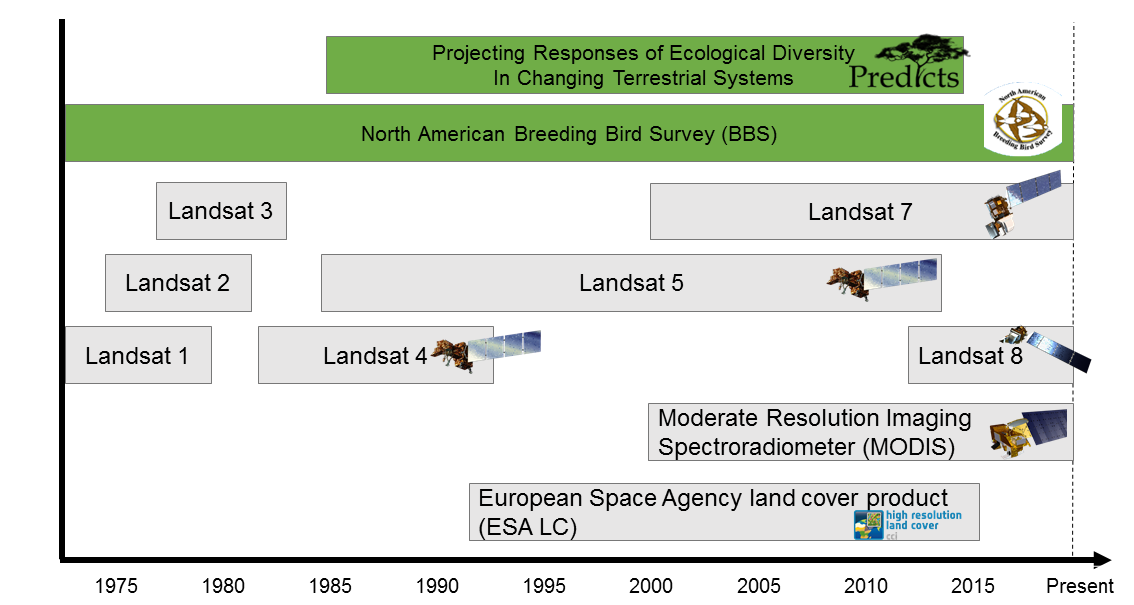
\includegraphics[width=1\textwidth]{chapter1/F01}
\caption{ Temporal coverage of biodiversity (green) and remote sensing (grey) datasets used in this thesis. Legacy Landsat missions (1-3) are shown for completeness only. }
\label{F01_01}
\end{figure}
% -------------------------------------------- %

Through technological advances humans have created a global spaceborne Earth observation system. The first satellite missions were used exclusively for military intelligence or weather observations. Since the mid-1970s satellite missions (Figure \ref{F01_01}), such as Landsat or later the Terra \& Aqua satellites with the Moderate Resolution Imaging Spectroradiometer (MODIS) sensor, were specifically designed to repeatedly photograph the Earth on a global scale \citep{Schaaf2002,Zhang2006,Kennedy2014}. These satellites carry highly sensitive sensors that measure the spectral reflectance from solar insolation. The near-infrared spectrum (Figure \ref{F01_02}\textbf{a}) has been recognized to be particularly useful for monitoring the photosynthetic activity of vegetation and can be quantified through “vegetation indices” \citep{Tucker1979,Tucker1981,Pettorelli2005,Jiang2008}. Differences in the dynamics of vegetation indices (Figure \ref{F01_02}\textbf{b}-\textbf{c}) can be used to identify land change globally. 

% ---------------- Figure 2 --------------------- %
\begin{figure}[htb]
\centering
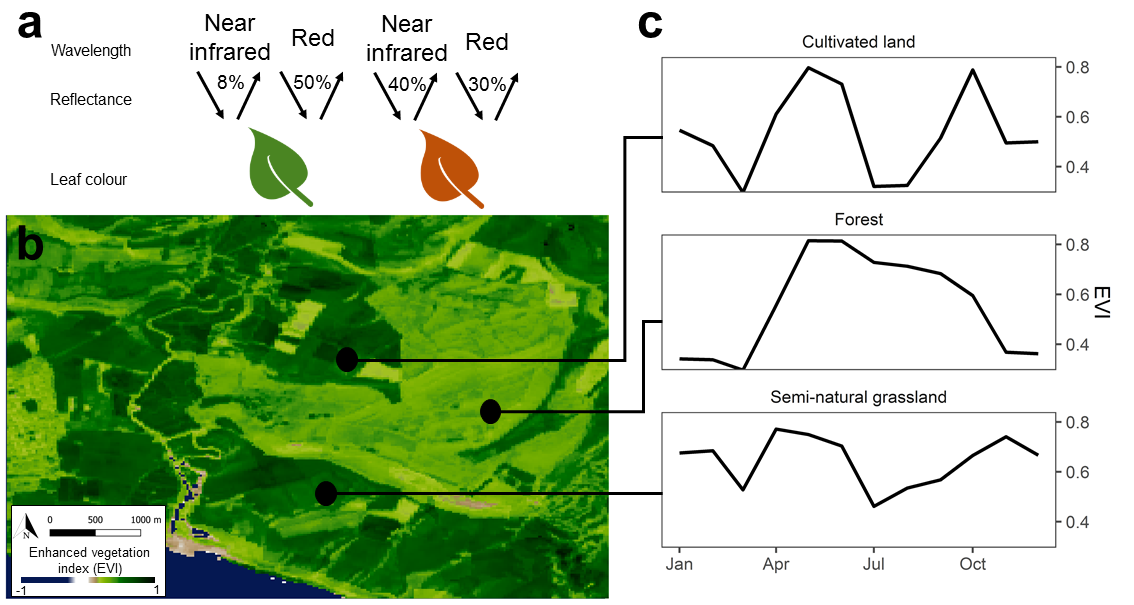
\includegraphics[width=1\textwidth]{chapter1/F02}
\caption{ (\textbf{a}) Schematic of how differences in spectral reflectances assist distinguishing leaf colour. (\textbf{b}) Map (Centre longitude: $0.165$\textdegree, latitude: $50.778$\textdegree) shows an annual maximum value composite (MVC) for 2018 of the Enhanced Vegetation Index (EVI) as calculated from the Landsat 8 mission. (\textbf{c}) Monthly MVC time series of three example sites (black points highlighted in \textbf{c}) of known land cover (cultivated land, forest, semi-natural grassland). }
\label{F01_02}
\end{figure}
% -------------------------------------------- %

Land change can be monitored using satellite-based remote sensing. A change on land can occur as either ‘conversion’ or ‘modification’, where the former is usually understood as “complete replacement of one land-cover type by another” \textendash\ \ie deforestation \textendash\ while the latter are “subtle changes” \textendash\ \ie agricultural intensification \textendash\ that affect the character of a land cover \citep{Lambin2003,Lambin2006}. Spatial estimates of the Earth’s land cover are commonly derived through a classification of remotely-sensed spectral reflectances \citep{DeFries1994,Hansen2000,DiGregorio2000}. However, these spatial estimates could often not be temporally compared because of classification biases and thematic inconsistencies \citep{VERBURG2011,Estes2018} and \textendash\ until recently \textendash\ little progress has been made to quantify land change globally. Novel algorithms and processing frameworks have been developed to quantify land change from temporal dynamics of spectral reflectances measuring photosynthetic activity \citep[Figure \ref{F01_02}\textbf{c}, ][]{Lhermitte2011,Gomez2016,Zhu2017}. With increasing availability and accessibility of satellite data \citep{Wulder2015} and computational power \citep{Gorelick2017} land changes have been quantified globally \citep{Hansen2013,Pekel2016,Li2018,Song2018}, creating new opportunities to  assess impacts of land change on biodiversity.   


\subsection{The impacts of past land change on local biodiversity}
\label{C01_0102}

% ---------------- Figure 3 --------------------- %
\begin{wrapfigure}{r}{0.5\textwidth}
  \begin{flushright}
    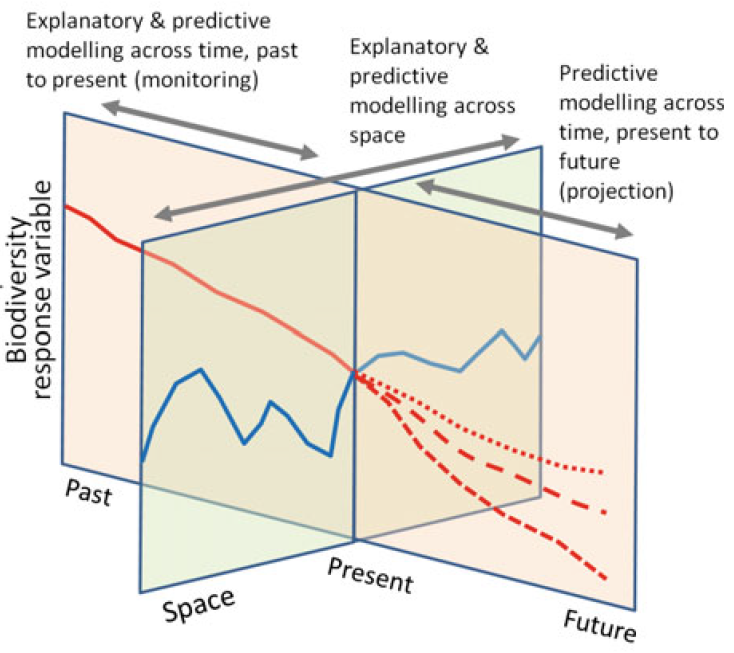
\includegraphics[width=.5\textwidth]{chapter1/F03}
  \end{flushright}
  \caption{ Schematic how a biodiversity response variable (red) can be estimated using environmental predictors (blue) in space and time. Adapted from \cite{Ferrier2017}. }
  \label{F01_03}
\end{wrapfigure}
% -------------------------------------------- %

Land changes can have immediate and/or delayed impacts on local biodiversity. They can act as disturbance affecting the stability of an ecosystem \citep{Pimm1984,Scheffer2003}, causing an immediate reduction in the number of species and individuals \citep{Nimmo2015,Ratajczak2018}. In addition, land changes can have delayed impacts on local biodiversity that persist for decades \citep{Martin2013,Moreno-Mateos2017} or centuries \citep{Vegas-Vilarrubia2011,McMichael2017}. Previous studies that investigated lasting influences of past land change \textendash\ varyingly described as “land-use history” or “landscape history” \citep{Bellemare2002,Foster2003,Ewers2013} or “management legacies” \citep{Perring2015} \textendash\ on biodiversity explained these influences through a number of mechanisms (Figure \ref{F01_04}, Table \ref{T01_01}).

% ---------------- Figure 4 --------------------- %
\begin{figure}[htb]
\centering
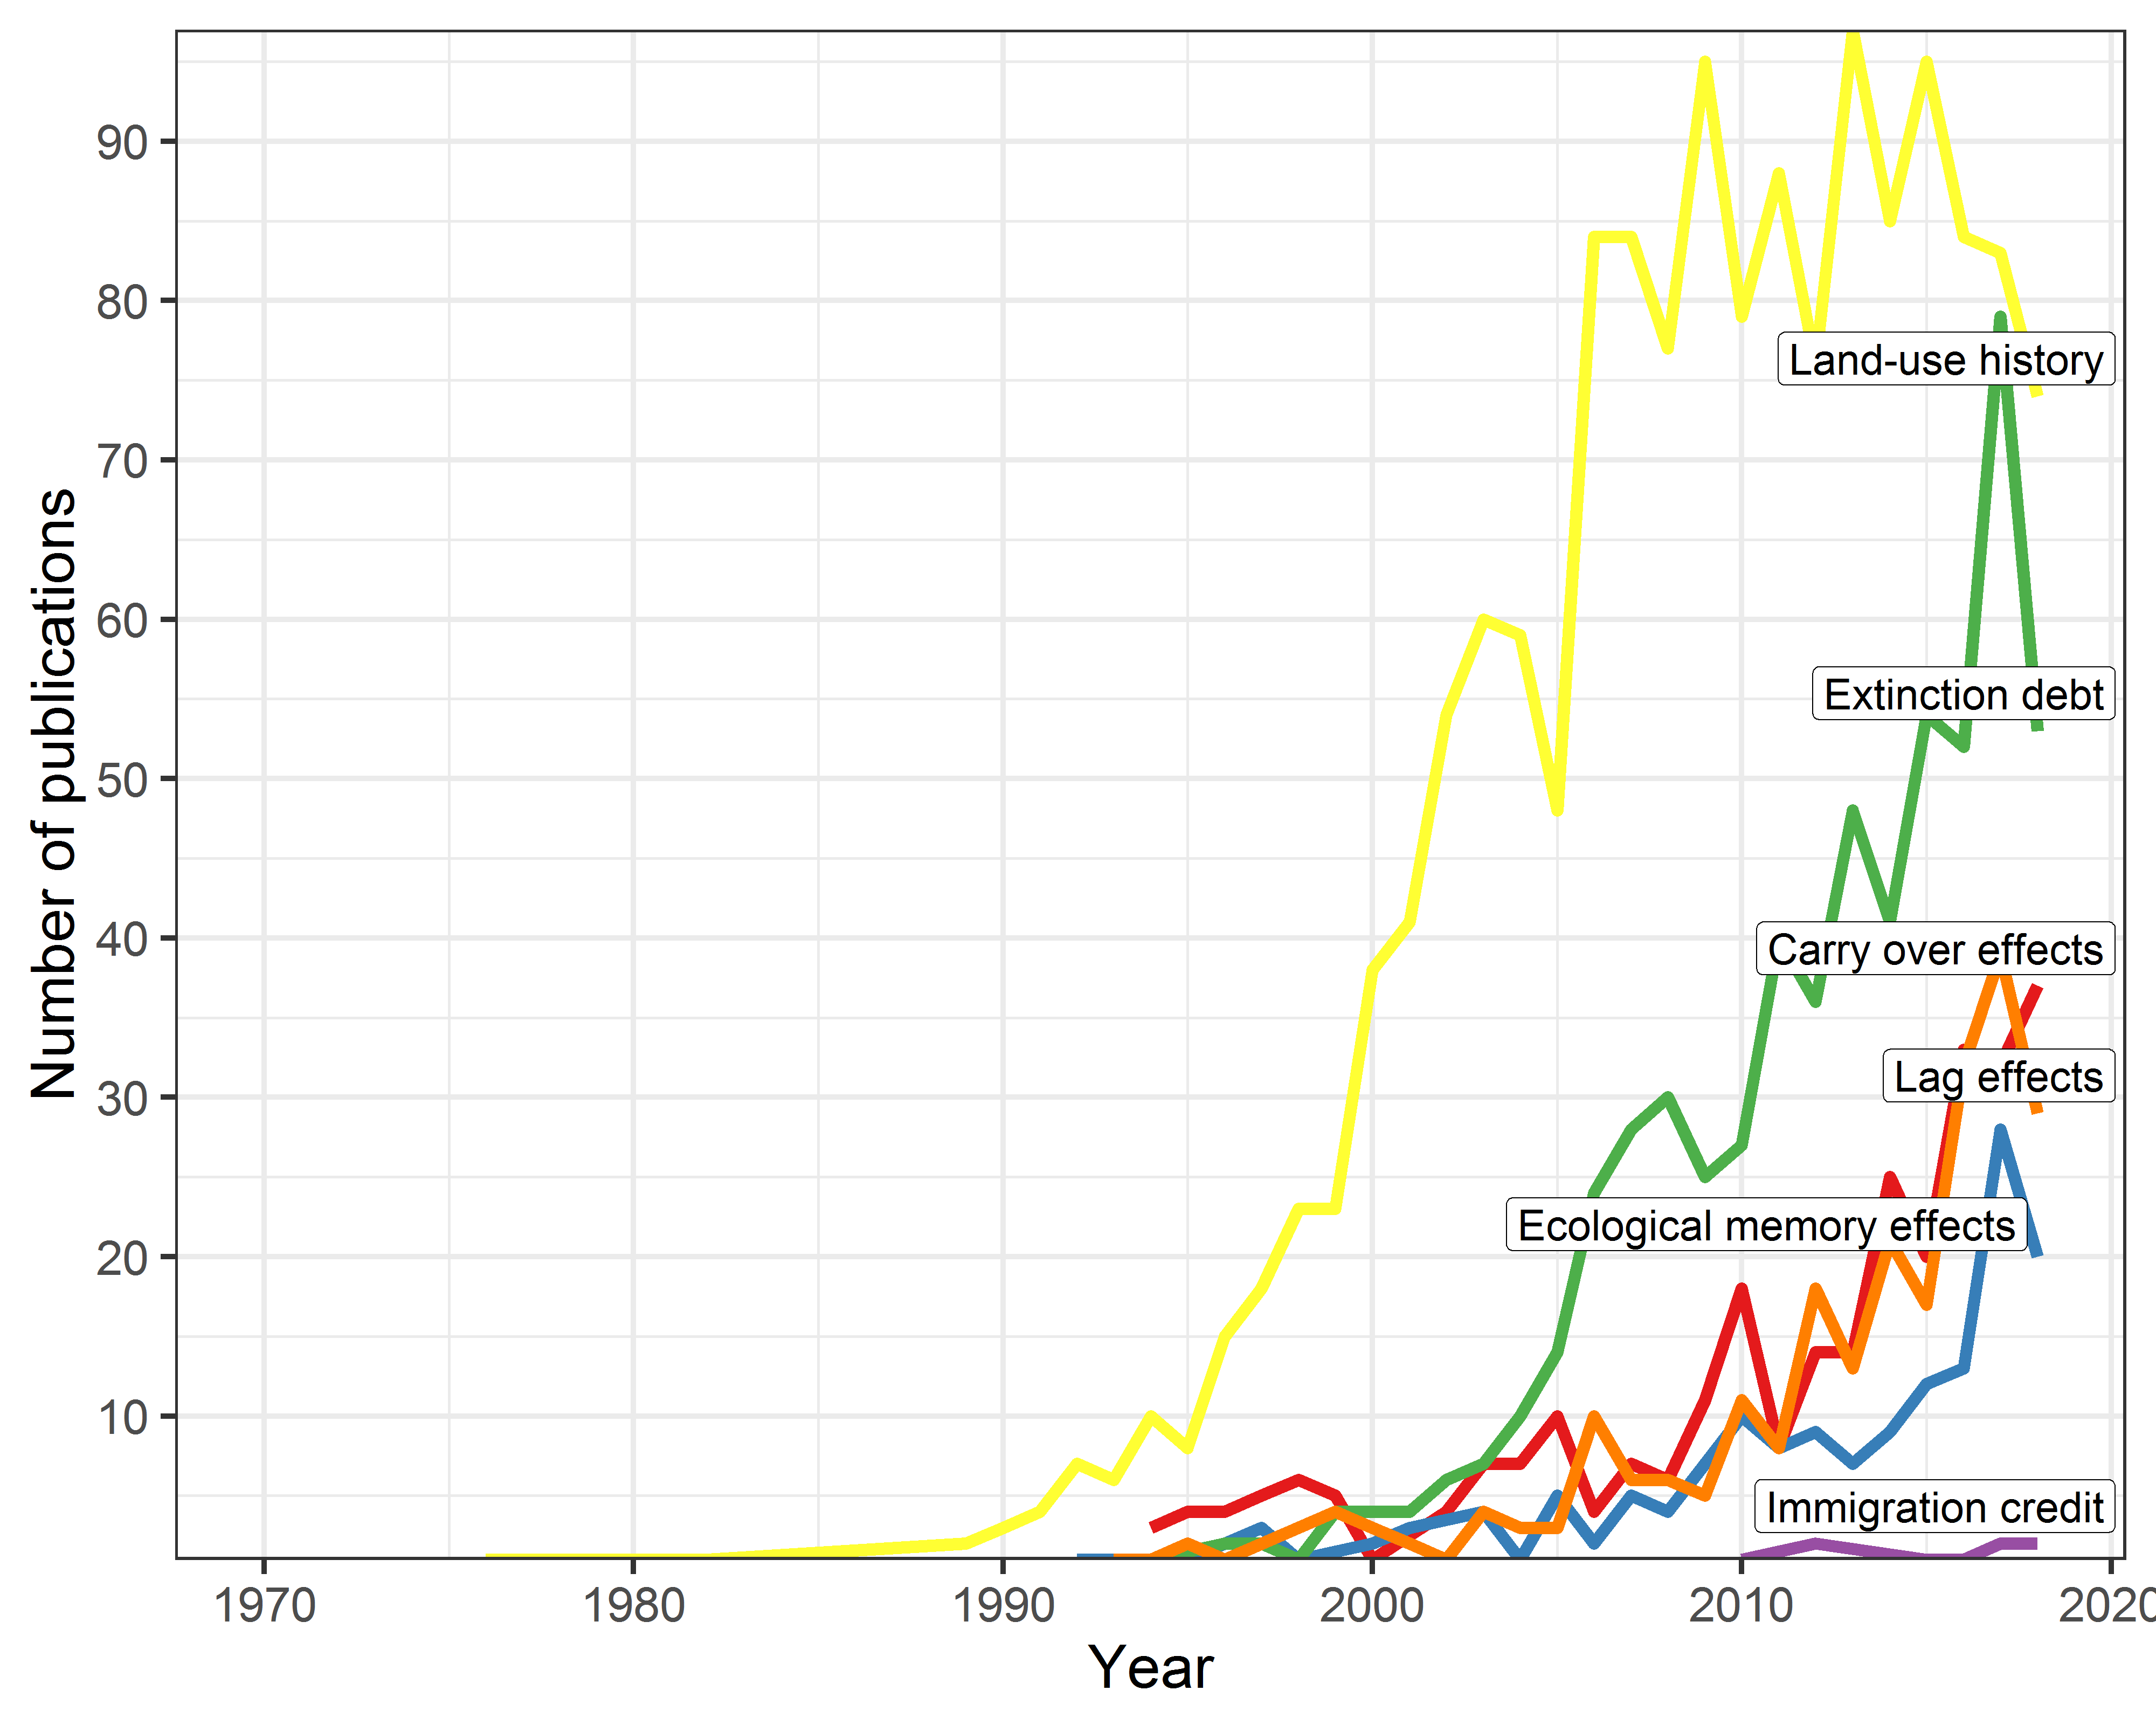
\includegraphics[width=1\textwidth]{chapter1/F04}
\caption{ Number of publications investigating terms and descriptions referring to biotic lag effects as queried from Web of Science\textsuperscript{TM} (WOS). A WOS search was conducted on the 5\textsuperscript{th} January 2019 limited to the Environmental sciences and ecological literature between 1900 and 2019 including as search topic “land-use histor*” (yellow), “extinction debt*” (green), “lag effect*” (orange), “carry*over effect*” (red), “ecological memory effect*” (blue) and “immigration credit*” (purple).  }
\label{F01_04}
\end{figure}
% -------------------------------------------- %

Several terms have been proposed to explain lasting impacts of past land change on local biodiversity (Table \ref{T01_01}). The term “extinction debt” describes the delayed extinction of species following a loss of habitat \citep{Balmford1996,Kuussaari2009,Wearn2012} and for many vertebrate species an extinction debt is usually “paid off” \textendash\ \eg the time until local population is fully extinct \textendash\ over a few years up to a century depending on the initial population size and species functional traits \citep{Halley2016}. Similarly, local biodiversity can also be influenced by an “immigration credit“, that is the delayed immigration of species from regional source populations after land change \citep{Jackson2010,Hylander2013}. Many species populations retain an “ecological memory” \citep{Peterson2002,Bengtsson2003,Ogle2015} of past land changes, reducing population growth and affecting species fitness and survival in subsequent years as “carry over” effect \citep{Harrison2011}. Collectively those terms can broadly be described as “biotic lag” effects (Table \ref{T01_01}), which are lasting or lagged effects of past changes in environmental factors that continue to influence present biodiversity. Knowledge about lasting impacts of land change can assist in planning management interventions \citep{Standish2014} and should be considered in broad-scale biodiversity models.  

Most existing regional and global assessments, models and scenarios of biodiversity \citep[\eg \ those included in the Intergovernmental Science-Policy Platform on Biodiversity and Ecosystem Services (IPBES) assessments, ][]{Alkemade2009,Pereira2010,Newbold2015} ignore lasting impacts of past land change. These assessments usually consider only concurrent differences in land-use/land-cover (Figure \ref{F01_03}) and may therefore partially misrepresent biodiversity change. Delayed impacts of past land change may accumulate together with other drivers \textendash\ such as climate change or species invasions \textendash\ of biodiversity change \citep{Essl2015,Essl2015a} potentially increasing the number of future species extinctions \citep{Dullinger2013}. To mediate the ongoing loss of biodiversity \citep{Mace2018}, robust estimates of the lasting impacts of land change on biodiversity need to be derived.

% ---------------- Table 1 ------------------- %
%\begin{landscape}
\begin{table}[ht]
\caption{Common terms and descriptions referring to lasting impacts of environmental changes on biodiversity}
\label{T01_01}

\newcolumntype{b}{X}
\newcolumntype{m}{>{\hsize=.6\hsize}X}
\newcolumntype{s}{>{\hsize=.4\hsize}X}

\begin{tabularx}{\textwidth}{ sbm }
\toprule
\textbf{Term} & \textbf{Description} & \textbf{Reference}   \\
\midrule

Land-use history  &  “Observed abiotic and biotic properties that are caused by past land use” & \citep{Foster2003,Perring2015} \\

Extinction debt & “The number of species committed to delayed extinction following a forcing event” &  \citep{Tilman1994,Kuussaari2009} \\

Immigration credit & “The number of species committed to delayed immigration following a forcing event” & \citep{Jackson2010} \\

Ecological memory & “The degree to which an ecological process is shaped by past modifications of the landscape, biotic and abiotic factors.” & \citep{Padisak1992,Peterson2002,Bengtsson2003,Ogle2015} \\

Carry-over effect & “Situation in which an individual’s previous history and experience explains their current performance in a given situation” & \citep{Harrison2011,OConnor2014} \\

Biotic lag &  Term summarizing the observed difference in biodiversity caused by lasting or lagged effects of past environmental changes  & \citep{DePalma2018} and this thesis   \\ \bottomrule

\end{tabularx}

\end{table}
% -------------------------------------------- %

\subsection{Linking satellite-based remotely-sensed land change with local biodiversity }
\label{C01_0103}

Remote sensing data can be useful for biodiversity models. Remotely-sensed land-surface conditions have been used to describe the biophysical state of species habitats \citep{Kerr2003}, identify critical life-history periods \citep{Pettorelli2005}, map species distributions \citep{He2015a} or as a proxy for predicting biodiversity patterns \citep{Rowhani2008,Rocchini2015,Hobi2017}. However, uncertainties remain in the usability of remote sensing data for different measures of biodiversity \citep{Oldeland2010}, for taxonomic groups \textendash\ where biodiversity measures are sometimes poorly correlated with photosynthetic activity \citep{Adler2011} or spectral dissimilarity \citep{Schmidtlein2017} \textendash\ or for many, previously unassessed geographic regions. Especially the temporal domain (Figure \ref{F01_02}\textbf{b}-\textbf{c}), including land change \textit{per se}, is often ignored \citep{Kennedy2014}. New frameworks are needed to establish links between remotely-sensed land change and local biodiversity.

Land change can be characterized by key attributes that may have varying impacts on local biodiversity (Figure \ref{F01_05}\textbf{a}). \cite{Watson2014} provided a conceptual framework that distinguishes between four attributes of land change: (\textbf{1}) The magnitude of land-change events, (\textbf{2}) the frequency of land-change events over time, (\textbf{3}) the time span since a land change occurred, and (\textbf{4}) the temporal sequence of land use and/or land cover categories (Figure \ref{F01_05}\textbf{a}). Ecological theory, experiments and simulations demonstrated that local biodiversity can be affected by these attributes (Figure \ref{F01_05}\textbf{b}). Land changes of larger magnitude are expected to affect biodiversity more \citep{Scheffer2001,Dornelas2010,Svensson2012,Ratajczak2018} and \textendash\ by removing poor dispersing \citep{Tilman1997} and specialist species \citep{Christensen2018} \textendash\ potentially reducing the stability of species assemblages \citep{Scheffer2001,Oliver2015,Hautier2015}. In many regions of the world, land changes vary in frequency \citep{Kleyer2007} impacting local biodiversity \citep{Valtonen2013,Lawson2015}, especially if those impacts accumulate in a short period of time \citep{Essl2015,Ratajczak2018}. Biodiversity measures can often recover to reference levels (\ie a temporal or spatial baseline) following land change, depending on the time passed \citep{Chazdon2003,Laurance2011,Martin2013}. Lastly, and commonly investigated, is the temporal sequence of land use and/or land cover types \citep{Harding1998,Chazdon2003,Foster2003}, where local biodiversity tends to be more altered at sites with past anthropogenic use. However, the impact of these four attributes of land change on local biodiversity has rarely been comparatively assessed globally and across taxonomic groups.

% ---------------- Figure 5 --------------------- %
\begin{figure}[htb]
\centering
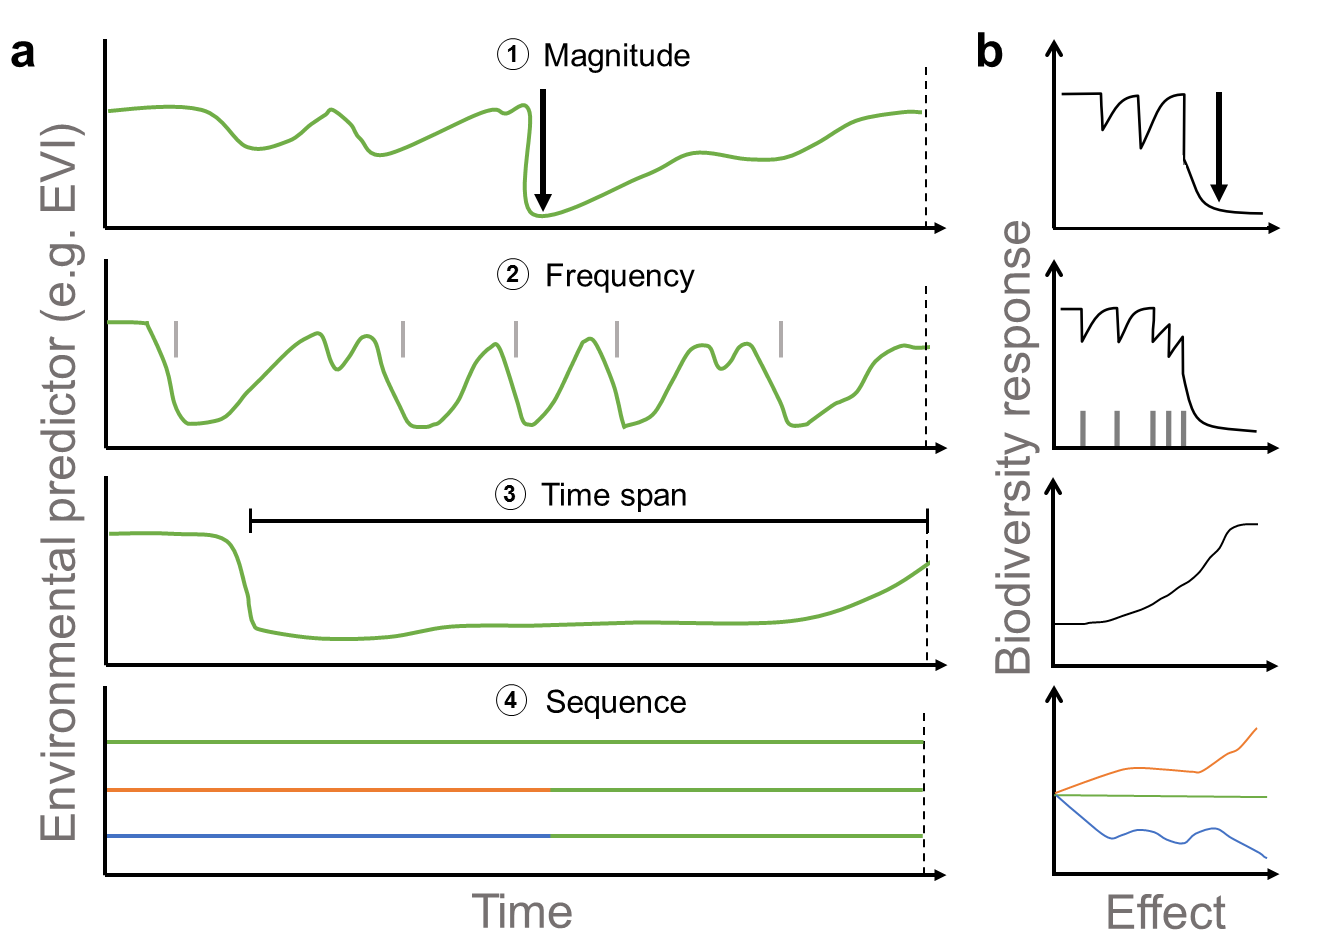
\includegraphics[width=1\textwidth]{chapter1/F05}
\caption{ (\textbf{a}) Conceptual framework \textendash\ inspired by \cite{Watson2014} \textendash\ how sites can differ by attributes of land change, namely (1) magnitude, (2) frequency, (3) time span and (4) sequence. Dashed lines indicate the start of biodiversity sampling with the y-axis representing an environmental predictor such as the Enhanced Vegetation Index (EVI). (\textbf{b}) Assumed response of biodiversity to varying land change attributes with x-axis indicating the strength of effect in units of each individual attribute.  }
\label{F01_05}
\end{figure}
% -------------------------------------------- %

\subsection{Thesis aims and structure}
\label{C01_0104}

The overall aim of my thesis is to investigate how local biodiversity is impacted by land changes globally and whether those impacts vary with attributes of land change  (Figure \ref{F01_05}). I do so by linking satellite-based remotely-sensed estimates of land change with measures of local biodiversity globally   (Figure \ref{F01_06}). The four main analytical chapters (Chapter \ref{C02}-\ref{C05}) of this thesis each address multiple of the four outlined attributes of land change (Figure \ref{F01_06}). They each serve as independent articles that have either been published, submitted or are in principle suitable for submission to an academic journal.

% ---------------- Figure 6 --------------------- %
\begin{figure}[htb]
\centering
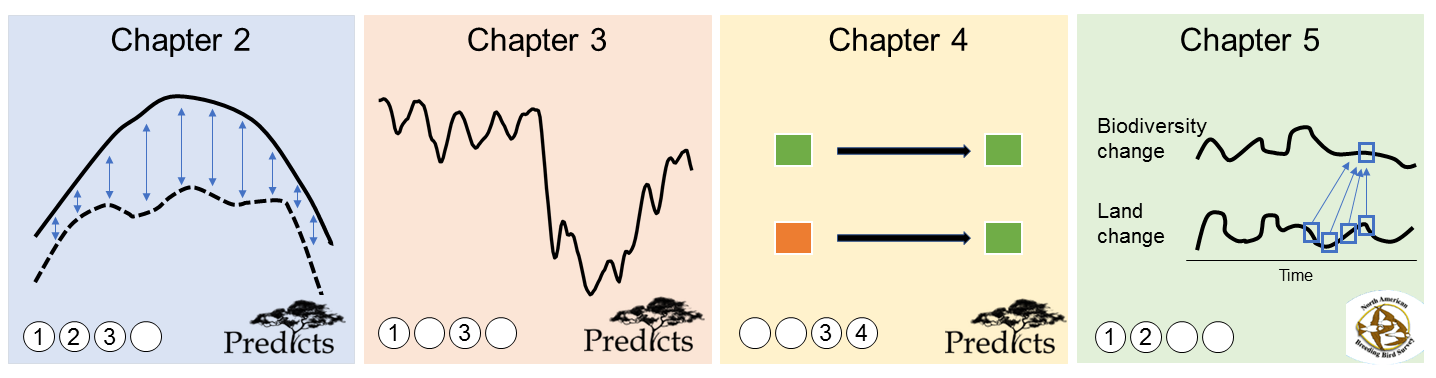
\includegraphics[width=1\textwidth]{chapter1/F06}
\caption{ Schematic outline of the four approaches (Chapter \ref{C02}-\ref{C05}) linking local biodiversity with remotely-sensed land change data, with lines and icons representing differences in intra-annual land dynamics (Chapter \ref{C02}), an abrupt land change of large magnitude (Chapter \ref{C03}), different land-cover sequences (Chapter \ref{C04}) and correlating temporal change in land and biodiversity observed at the same sites (Chapter \ref{C05}). Numbers in circles at the bottom left (1-4) indicate which attributes of land change from \cite{Watson2014} are considered in each approach (see Figure \ref{F01_05}\textbf{a}), while logos indicate the biodiversity data used (PREDICTS or United States BBS data). }
\label{F01_06}
\end{figure}
% -------------------------------------------- %

Chapter two assesses whether considering past land-surface conditions in the six years before biodiversity sampling can assist in explaining differences in local biodiversity. I developed an analytical framework that captures all differences between time series of remotely-sensed land-surface conditions \textendash\ such as land changes with varying magnitude or inter-annual frequency \textendash\ in a single metric, which was then linked with differences in species assemblage composition across taxonomic and functional groups globally. 

The third chapter focusses on how abrupt land changes \textendash\ characterized by shifts in magnitude or trend and varying time passed \textendash\ continue to influence local biodiversity. I assembled time series of Landsat imagery globally (Figure \ref{F01_01}\textbf{a}) and subjected them to a change-detection algorithm to detect abrupt land changes. A hierarchical analysis was conducted to assess if and how strongly local biodiversity differs between sites with and without a land change in the past. The assumption is that local biodiversity is more affected by abrupt land changes of greater magnitude that occurred more recently.

In chapter four I investigated how local biodiversity differs between sites with varying land-cover sequences of land cover change as derived from a global, temporally consistent land-cover product for the years 1992 to 2015. The assumption is that local biodiversity is higher at sites with a past land-cover change compared to those without, if the preceding land cover was less anthropogenically modified. In addition, this chapter investigates how past land-cover sequences can influence global and national biodiversity projections and argues for including estimates of past land change in biodiversity projections.

In contrast to previous chapters, in the fifth chapter I investigate if local biodiversity change can be linked to landscape-wide land changes. Estimates of bird diversity change from repeated breeding bird surveys (BBS data, Figure \ref{F01_01}) were correlated with estimates of preceding and concurrent land change at the landscape scale quantified from time series of Landsat imagery. I furthermore investigate whether the explanatory power of landscape-wide land changes on bird diversity change varies in space, time and across functional groups of bird species. The assumption is that bird diversity declines more in landscapes with a greater proportion of land changes.

The thesis concludes with the sixth chapter, which provides a synthesis of the presented work, discusses all findings in relation to previous studies, and mentions shortcomings and promising directions for future research.

\clearpage
%\bibliography{content/01Chapter}

%\appendix
%\begingroup
%  Blank

%\endgroup

  \chapter{ Local species assemblages are influenced more by past than current dissimilarities in photosynthetic activity}
\label{C02}
%\addcontentsline{toc}{chapter}{Chapter 2}
%\markboth{}{Local species assemblages are influenced more by past than current dissimilarities in photosynthetic activity}

Most land on Earth has been changed by humans and past changes of land can have lasting influences on current species assemblages. Yet few globally representative studies explicitly consider such influences even though auxiliary data, such as from remote sensing, are readily available. Time series of satellite-derived data have been commonly used to quantify differences in land-surface conditions such as vegetation cover, which will among other things be influenced by anthropogenic land conversions and modifications. Here we quantify differences in current and past (up to five years before sampling) vegetation cover, and assess whether such differences differentially influence taxonomic and functional groups of species assemblages between spatial pairs of sites. Specifically, we correlated between-site dissimilarity in photosynthetic activity of vegetation (the Enhanced Vegetation Index) with the corresponding dissimilarity in local species assemblage composition from a global database using a common metric for both, the Bray-Curtis index. We found that dissimilarity in species assemblage composition was on average more influenced by dissimilarity in past than current photosynthetic activity, and that the influence of past dissimilarity increased when longer time periods were considered. Responses to past dissimilarity in photosynthetic activity also differed among taxonomic groups (plants, invertebrates, amphibians, reptiles, birds and mammals), with reptiles being among the most influenced by more dissimilar past photosynthetic activity. Furthermore, we found that assemblages dominated by smaller and more vegetation-dependent species tended to be more influenced by dissimilarity in past photosynthetic activity than prey-dependent species. Overall, our results have implications for studies that investigate species responses to current environmental changes and highlight the importance of past changes continuing to influence local species assemblage composition. We demonstrate how local species assemblages and satellite-derived data can be linked and provide suggestions for future studies on how to assess the influence of past environmental changes on biodiversity.

\section{Introduction}
\label{C02_01}
Throughout the Earth's history, land has changed constantly by a combination of natural and anthropogenic forces. Palaeontological evidence indicates that humans have transformed approximately 75\% of the land at least once \citep{Ellis2010,Ellis2011}, with changes in many land-surface conditions, such as vegetation cover, accelerating since the beginning of the industrial revolution \citep{Lambin2006,Steffen2015}. Changes in vegetation cover may be caused by climatic factors, such as CO\textunderscript{2} fertilization or altered precipitation patterns \citep{Zhu2016}, or anthropogenically caused land conversions, such as deforestation, re- and afforestation \citep{Dupont2003,Hansen2013,Muller2014} or land modifications, such as degradation, intensification \citep{Gibbs2015,Rufin2015} or return to less intensive forms of land use \citep{Zomer2016}. Over time, these changes have shaped both land and species assemblages in complex ways \citep{Foster2003,Watson2014,Perring2015}.

Most global meta-analyses investigating the influence of differences in vegetation cover on species assemblages have assumed that any difference in vegetation cover at the time of biodiversity sampling is the dominant influence
\citep{Stein2014, Newbold2014b, Newbold2015, Alroy2017}. However, this assumption might be incorrect as assemblages can be heavily influenced by legacy effects of past changes in vegetation cover \citep{Foster2003, Watson2014, Ogle2015, Perring2015}. For the recent past (\eg, up to five years prior to biodiversity sampling), ecological memory or carry-over effects, \ie the capacity of past events to influence present and future ecological assemblages \citep{Harrison2011, OConnor2014, Ogle2015}, have been proposed as mechanisms that shape species assemblages. These effects can arise through site-specific environmental factors, for instance altered conditions because of agricultural practices \citep{Perring2015,Perring2018} or different sequences and successional recovery from changes in past vegetation cover \citep{Johnson2008,Walker2010,Watson2014}. No detailed global analysis to date has explicitly considered the influence of both current and past differences in vegetation cover on current species assemblages.

While some differences in species assemblages can be traced back to changes in vegetation cover in the late quaternary \citep{Vegas-Vilarrubia2011,McMichael2017}, there is some evidence that changes in vegetation cover in the more recent past can influence plant \citep{Jakovac2016}, invertebrate \citep{Valtonen2013} or vertebrate assemblages \citep{Newton2014, Cole2015, Graham2015}. However, this has — to our knowledge — not been assessed comparatively across multiple taxonomic groups. Furthermore, it is likely that species with specific traits, such as certain body size and/or trophic level, may be differentially affected by past changes in vegetation cover because of differences in their metabolic rate (for animals), longevity or dispersal abilities \citep{Sutherland2000, Brown2004, Speakman2005,Thomson2011,DePalma2015}. Depending on the type and magnitude of a past changes in vegetation cover (as a proxy for land-surface changes) plant assemblages can either be dominated by small, fast sprouting or taller, nutrient-demanding species \citep{Jakovac2016,Perring2018}. Until now, our understanding of the influence of past differences in vegetation cover on species assemblages has been limited to case studies focused on specific regions or certain taxonomic and functional groups. However, a recently published globally representative dataset on species assemblages of broad taxonomic coverage \citep{Hudson2016} and globally available satellite-derived data enable us to consider explicitly both current and past differences in land-surface conditions.

Satellite-derived data can provide internally consistent estimates of how land differs across time and space \citep{Pettorelli2005, Kennedy2014}. Land-surface conditions such as photosynthetic activity of vegetation can be quantified using spectral indicators from satellite-derived data \citep{Gamon1995, Zhang2006}. Changes in photosynthetic activity of vegetation can be related to both climatic \citep{Fensholt2012, Zhu2016} and anthropogenic factors such as land conversions and modifications \citep{Lambin2003, Muller2014}. Subtle differences in vegetation dynamics (as measured by various satellite-derived vegetation indices), such as faster greening rate or differing seasonal amplitude, between years have been used to characterize land change \citep{Lambin1994, Linderman2005, Lupo2007}. Recent studies have used such differences to identify changes in land use such as pasture use intensity \citep{Rufin2015}, fallow periods in croplands \citep{Estel2015, Tong2017}, small-scale deforestation \citep{DeVries2015b} and broad scale land degradation and intensification \citep{deJong2011,Muller2014}. Dissimilarity metrics describing the entirety of recent land history (\eg including both differences in land use and land cover as well as climatic and site-specific factors) can be calculated between spatial pairs of time series as the overall dissimilarity in photosynthetic activity \citep{Linderman2005, Lhermitte2011}. Increasingly such methods have been linked to dissimilarity in local species assemblage composition \citep{Rowhani2008, Goetz2014, Nieto2015, Hobi2017}, however few studies have explicitly distinguished between current and past dissimilarity in photosynthetic activity.
	
Here we use a time series dissimilarity metric (the Bray-Curtis index) to quantify dissimilarity in a land-surface attribute, e.g. photosynthetic activity of vegetation, among spatial pairs of sites in the Projecting Responses of Ecological Diversity In Changing Terrestrial Systems (PREDICTS) dataset \citep{Hudson2016}. We explicitly distinguish between dissimilarity in current and past photosynthetic activity (BC\textunderscript{EVI}), defined here as the five years prior to the ‘current’ year, and assess how they influence compositional dissimilarity (BC\textunderscript{Biodiversity}) between species assemblages among paired sites. This pairwise comparison approach allows us to investigate (\textit{i}) the overall influence of past relative to current dissimilarity in photosynthetic activity on species assemblages where we hypothesize that the influence of past dissimilarity increases with longer past periods considered. Furthermore, we investigate (\textit{ii}) whether different taxonomic groups respond differently to past dissimilarity in photosynthetic activity, and (\textit{iii}) if species with particular functional characteristics, \ie, those that are smaller and/or more vegetation-dependent, are more affected by past dissimilarity in photosynthetic activity than others. 


\section{Data and Methods}
\label{C02_02}
\subsection{Remotely-sensed data}
\label{C02_0201}
A temporal profile of spectral reflectance values was derived from the Moderate Resolution Imaging Spectroradiometer (MODIS) sensor on board NASA’s Terra and Aqua satellites. Since the year 2000, MODIS has provided continuous spectral data of medium-scale resolution (nominal \textasciitilde500 m resolution) with high temporal revisit rates (a global image collection is taken every day) \citep{Schaaf2002}. We used the Bidirectional Reflectance Distribution Function and Albedo (BRDF) product (MCD43A4.005), which aggregates the highest quality daily spectral reflectance values into 8-day composites of seven spectral bands \citep{Schaaf2002}. Google Earth EngineTM was used to download and process temporal profiles of all spectral bands for each site \citep{Gorelick2017}. We calculated a spectral index measuring photosynthetic activity (the two-band Enhanced Vegetation Index – EVI; \cite{Jiang2008}), which is based on a ratio between the near-infrared (nir, 841-876 nm) and red (red, 620-670 nm) spectral band \( EVI = 2.5 * \frac{(nir - red)}{(nir + 2.4 * red + 1)} \). We used the EVI as it has been designed to reduce atmospheric contamination and not to saturate in high biomass regions such as tropical rainforests \citep{Huete2002,Jiang2008}. We applied the following pre-processing steps (also see flowchart in Appendix Figure \ref{SI02_01}) to the nir and red BRDF bands individually to fill missing observations and filter out extreme data points. 

First, we detected and removed extreme outliers in the BRDF data that may have been introduced by cloud shadows, atmospheric haze, inversion errors or sensor failures. We calculated the absolute difference of all values from the median relative to the total median absolute deviation (MAD) of all values \citep{Leys2013}. Pixels which were more than a conservative threshold of two units deviation \citep[but see][]{Leys2013} away from the MAD as well as greater than 99\% of all other difference values were set to missing. This data-defined threshold removed only the most extreme outliers and retained fluctuations that are within the bounds of median conditions. We chose this procedure rather than using the MODIS BRDF quality data set (stored in the separate MCD43A2.005 product) to maintain the maximum number of observations assuming that bad quality inversions of the BRDF product are filtered and smoothed out by subsequent pre-processing steps.

Second, we interpolated missing values using a Kalman filter, a smoother for estimating missing data points based on preceding data \citep{Kalman1960}. Previous studies have shown that Kalman filters perform well in filling gaps in BRDF time-series especially in data-poor regions \citep{Samain2008}. The best model for the Kalman filter for a given time-series was estimated using the “forecast” R package (“auto-arima” function) by selecting the model with the lowest Akaike Information Criterion (AIC) \citep{Hyndman2008}. We only interpolated consecutive gaps $\leq 40$ days (\ie five consecutive 8-day BRDF composites) as longer interpolations would reduce our ability to detect short-term changes in photosynthetic activity.  We excluded all time-series from further analyses with more than 50\% remaining missing data (average proportion of missing data = 6.32 $\pm$ 10.31\%) in the time period considered (see Appendix Figure \ref{SI02_02}). 

Lastly, we applied a Savitzky-Golay filter (filter length = 5, “signal” R-package) to reduce the amount of random noise remaining in the time series, but retain small abrupt changes that might occur \citep{Joensson2004}. The Savitzky-Golay filter performs well relative to other smoothing techniques in removing noise \citep{Kandasamy2013}. Our pre-processing steps aimed to remove influential outliers and random noise from each time series, but we cannot rule out that some non-informative noise has remained in the time series. From these pre-processed BRDF data we calculated the EVI for each 8-day composite \citep{Jiang2008}.

\subsection{Species assemblage data}
\label{C02_0202}
We used data on species’ abundance within local-scale assemblages from the PREDICTS database \citep[downloaded on 3 February 2016, see \ref{SI02_01}]{Hudson2016}, which is the largest global database investigating anthropogenic impacts on terrestrial species assemblages to date. The PREDICTS database has collated local-scale species assemblage records from the published literature (henceforth “sources”) comparing observations among at least two localities (henceforth “sites”) with differing land use or related pressures. Sources in the PREDICTS database having multiple sampling methodologies and taxonomic groups were split accordingly into different “studies”. Wherever sampling effort differed among sites within a study, we followed the approach of \cite{Newbold2014b} and adjusted abundance values assuming that recorded abundance increase linearly with effort. Each study was assigned to one of six higher taxonomic groups based on the sampled species identity (Plants, Invertebrates, Amphibians, Reptiles, Birds and Mammals). We grouped plants and invertebrates into single individual groups as there were insufficient data to divide them into smaller groups (\eg, functional divisions such as flying vs ground-living insects). Studies of fungi were dropped from the analyses because of insufficient data.

Of the 25224 sites with abundance data, we removed 6109 sites because their sampling durations spanned more than a year or because the start of biodiversity sampling differed by more than three months among sites within a study. This was done to avoid seasonal effects confounding any link between species assemblage composition and remote-sensing derived estimates. Furthermore, we removed 10248 sites from studies that sampled biodiversity before the 18th of February 2006 to ensure MODIS data availability for at least five years prior to biodiversity sampling. We chose to use a five-year period to allow sufficient MODIS coverage (since year 2000) for the majority of studies in the PREDICTS database (median biodiversity sampling start date = 2007-07-17). In total 8867 sites were suitable to be linked with MODIS remote-sensing data.

The spatial extent of biodiversity sampling at PREDICTS sites typically differs from the resolution of MODIS data. We used the Maximum Linear Extent (MLE) information within the PREDICTS database, which summarises the spatial extent of sampling within a study in metres \citep{Hudson2016}. Sites from a few studies had large MLE (up to 40 km) and after visual exploration, we decided to keep only those sites that were within the 99\% quantile of all MLE values (MLE < Q99 = 3000 m, removing 249 sites). Some studies had missing MLE information (25\% of all studies with abundance data, 728 sites), where no MLE estimate could be obtained during the PREDICTS data curation \citep{Hudson2016}. We filled missing MLE information with the average MLE estimate of each taxonomic group with corresponding sampling method, and any remaining missing MLE, for which no other combination of taxonomic group and sampling method had MLE estimates, with the average MLE for each taxonomic group. We tested the robustness of this assumption by removing 25\% of the existing MLE estimates at random and found interpolated MLE values to be reasonably accurate (r = 0.73, p < 0.001). We used the centre coordinates for the rest of the sites (mean MLE $\pm$ SD = 256.52 m $\pm$ 437.93 m) as their spatial extent roughly matched the nominal spatial resolution of the MODIS data (\textasciitilde 500 m). 

We excluded studies from our analyses where all study sites fell within a single MODIS grid cell, to suit our hierarchical statistical approach (see below). Some sites within a study could fall into the same MODIS grid cell, therefore for all further analyses we randomly selected one site per study per grid cell 100 times (See section on analysis – pairwise differences below for description of permutation procedure and Appendix Figure \ref{SI02_03} for a schematic), resulting in 100 different subsets that we used for all further analyses. Our final dataset included data from 198 studies with 4053 sites per permutation and model covering all major continents and most taxonomic groups (Figure \ref{F02_01}).

% ---------------- Figure 1 --------------------- %
\begin{figure}[ht]
\centering
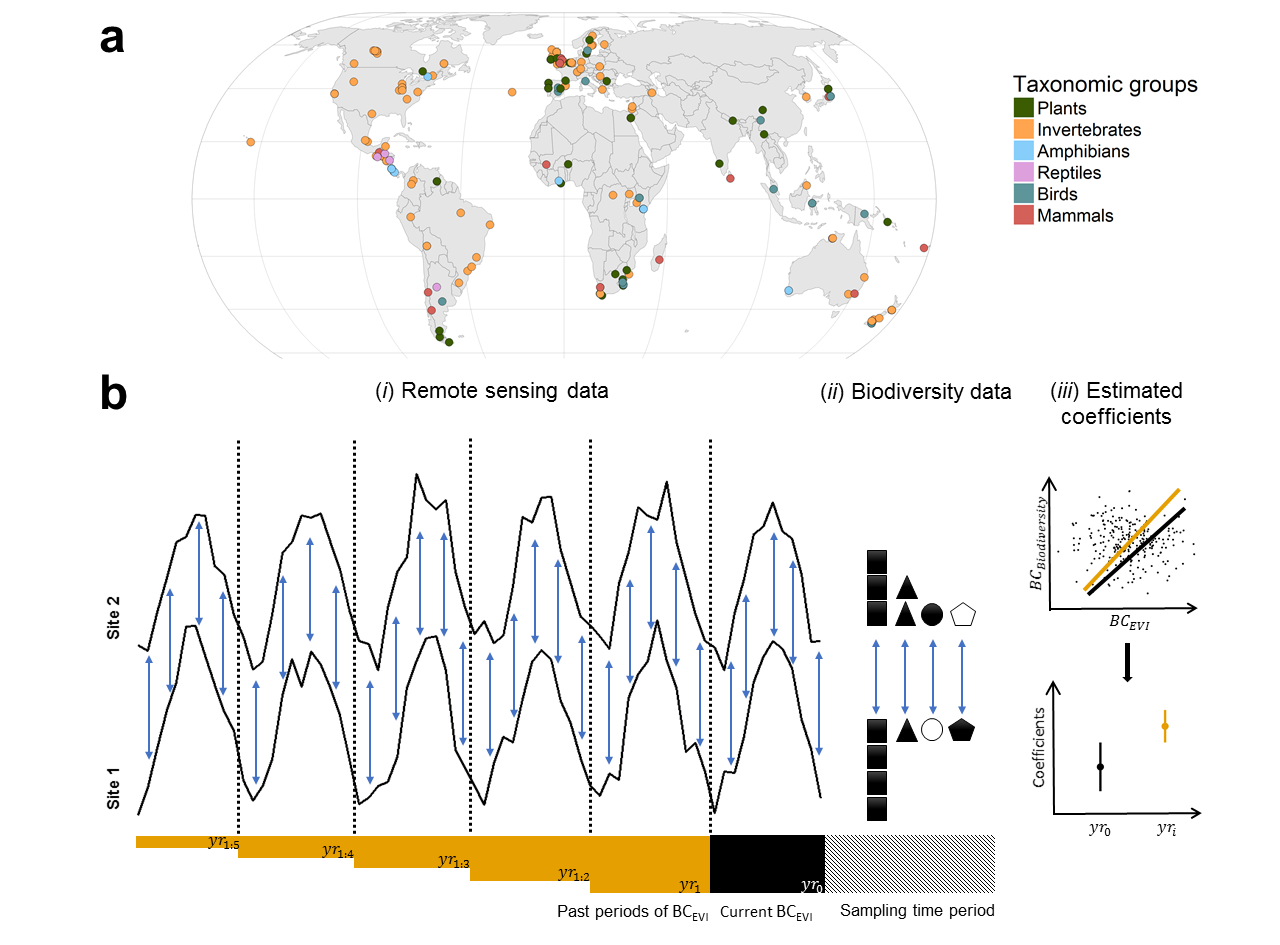
\includegraphics[width=1\textwidth]{chapter2/F01}
\caption{ (\textbf{a}) Locations of 198 species assemblage studies (centroid of each study) coloured by taxonomic group. (\textbf{b}) Diagram of the modelling approach to investigate influences of current and past dissimilarity in photosynthetic activity on species assemblages. The Bray-Curtis index (BC\textunderscript{EVI}) was calculated between pairs (blue arrows) of remote-sensing time series (black solid lines) and of species assemblages (BC\textunderscript{Biodiversity}) collected at paired sites. Independent statistical models were constructed for both current (i - black) and past BC\textunderscript{EVI} of varying length (ii - orange) and their model effects compared (iii – Estimated fixed effects).}
\label{F02_01}
\end{figure}
% -------------------------------------------- %

\subsection{Species trait compilation}
\label{C02_0203}
A species’ size and trophic level are two of the most basic traits for understanding differences in species assemblage structure \citep{Speakman2005,Terborgh2015}. We classified studies into size and trophic bins based on a simple majority: small (>0-9 g animal body mass or > 0-9 cm plant height), medium (10 – 99 g or 10-99 cm) or large species (>= 100 g or >= 100 cm), or predominantly herbivore, omnivore, carnivore or detritivore species, by estimating the dominant number of species (simple sum of measurement) within a study. Studies with species of predominantly unknown size or trophic level were removed from the analysis. We thus classified entire studies to the dominant bins as each study’s methodology would likely constrain the average size of animals or plants that can be observed. Data on average adult body mass (in g) were collected for mammals \citep{Jones2009} and birds \citep{Myhrvold2015}, while for plants we used height (in cm) data from the TRY database \citep{Kattge2011}. The estimates of species trophic levels originate from \cite{Kissling2014}, \cite{Wilman2014} and other sources of the literature for invertebrates (obtained from Laura Bentley, Imperial College London, UK). For species for which size or trophic level data were unavailable, we used the genus-wide average for size and the most common trophic level (at least 95\% of all species with data within a genus). We excluded studies (N=8) from further analyses where no clear majority of species (> 50\%) could be assigned to one of the bins (Appendix Figure \ref{SI02_04}), leaving a total of 65 studies with size information and 130 studies with trophic information. 

\subsection{Analysis - Pairwise dissimilarity}
\label{C02_0204}
We linked dissimilarity in photosynthetic activity of vegetation with compositional dissimilarity in species assemblages globally. Specifically, we examined the differential influence of “current” (yr\textunderscript{0}, as the 365 days prior to species assemblage sampling) and “past” (yr\textunderscript{i}, the i years prior to the current year, where $i = 1,..,5$) dissimilarity in photosynthetic activity between spatial pairs of sites (Figure \ref{F02_01}\textbf{b}, Appendix Figure \ref{SI02_03}). We separately considered past periods of increasing lengths (in years, so yr\textunderscript{1}, yr\textunderscript{1:2}, yr\textunderscript{1:3}, yr\textunderscript{1:4}, yr\textunderscript{1:5}). For example, if species assemblage sampling was conducted from the 1st of April until the 15th of July 2008, yr\textunderscript{0} was the 365 days prior to 1st of April 2008, i.e. 1st April 2007 – 31th March 2008, and past i years as the period (number of full years i) before April 1st 2007.

We used the pairwise Bray-Curtis (BC) index, frequently used in community ecology studies, as a metric to quantify dissimilarity in species assemblage composition between sites \citep{Bray1957,Faith1987,Su2004}. We also considered the binary version of the BC index, the S\o rensen similarity index, to assess whether our results are robust to metric choice. The BC index is a modified Manhattan distance, where the summed distances between values are standardised by the summed values of each site, thus quantifying pairwise dissimilarity from 0 (completely similar) to 1 (entirely different). We used the BC index to measure compositional dissimilarity in local species assemblages (BC\textunderscript{Biodiversity}) between sites within a PREDICTS study. We also applied the BC index to the EVI time series (BC\textunderscript{EVI}) to characterize the dissimilarity between sites in (inter- and intra-annual) vegetation dynamics measured through a proxy representing photosynthetic activity of vegetation in current (yr\textunderscript{0}) and past years (yr\textunderscript{i},where $i = 1,..,5$), which to our knowledge is the first time the BC index has been applied to assess dissimilarity between remotely-sensed time series.

The BC index is calculated between two pairs of sites with PREDICTS species assemblage records or two EVI time-series from sites x and y as follows: 
\begin{equation*}
    BC_{xy} = \frac{( \sum_{k=1}^{n} |x_k - y_k  | )}{ (\sum_{k=1}^{n} x_k + \sum_{k=1}^{n} y_k )}
\end{equation*}
For species assemblages, $x$ and $y$ are the abundances of observed species (n = total number of species) at both sites (non-occurring species were assumed to be absent and set to zero), while for the EVI time series x and y are observed EVI values on the same date (n = total number of dates) in the time series at both sites. The BC\textunderscript{EVI} was calculated on either single or multiple years (yr\textunderscript{i},where $i = 1,..,5$) of EVI time series (Figure \ref{F02_01}\textbf{b}, Appendix Figure \ref{SI02_03}).

Compared to other metrics quantifying dissimilarity between time-series based on remotely-sensed data \citep{Lhermitte2011} the BC\textunderscript{EVI} index has the advantages of (\textbf{a}) taking the actual spectral values as well as distance between them into account, meaning it can be compared between different land-cover types, and (\textbf{b}) using the same method for assessing dissimilarity between species assemblages and between remote-sensing observations. In remote-sensing terms, for any vegetation index (such as EVI), the BC\textunderscript{EVI} index can be interpreted as a measure of absolute differences between two sites in the amount and timing of photosynthetic activity scaled by the total amount of photosynthetic activity available. By calculating the BC\textunderscript{EVI} index on temporal profiles of EVI measurements, we incorporate all differences in EVI between two sites into a single dissimilarity metric. No further scaling has been done as range and unit of the BC\textunderscript{EVI} index values were identical for current and past BC\textunderscript{EVI}.

\subsection{Analysis - Statistical modelling}
\label{C02_0205}
The aim of the statistical modelling is to estimate the influence of current and past BC\textunderscript{EVI} on the BC\textunderscript{Biodiversity} (Figure \ref{F02_01}\textbf{b}). For different time periods (0-5 years) we estimated this influence using separate models rather than an interaction term as current and past BC\textunderscript{EVI} were highly collinear (Random permutation pick: Pearson’s r > 0.9, df = 4046, p < 0.001). A hierarchical modelling approach using generalized linear mixed models (GLMMs) with Gaussian link function was used to fit models of current and past BC\textunderscript{EVI} independently for each time period, taxonomic group, size and trophic bins. GLMMs account for differing sampling methodologies among the PREDICTS studies, by including the “study” as a random intercept in all models. We also allowed the effect of current and past BC\textunderscript{EVI} to vary for each study by incorporating it as a random slope. From each model, we obtained the fixed effects (estimated slope) of the predicted BC\textunderscript{Biodiversity} per unit of current and past BC\textunderscript{EVI}.
	
As we are primarily interested in the influence of past BC\textunderscript{EVI} (of different periods) on differences in BC\textunderscript{Biodiversity}, we incorporated the influence of current BC\textunderscript{EVI} by transforming the average past BC\textunderscript{EVI} effects (across all permutations) relative to current effects $\frac{Past}{(Current - 1)}$. The resulting ratio describes whether the explicit influence of past BC\textunderscript{EVI} on BC\textunderscript{Biodiversity} is larger (> 0) or smaller (< 0) than the influence of current BC\textunderscript{EVI} (Figure \ref{F02_02}). The precision estimates (predicted standard errors) of the effect of past BC\textunderscript{EVI} were also transformed relative to the precision estimates of current BC\textunderscript{EVI} $\frac{(Imprecision_{past})}{(Imprecision_{current})}$. This helps to visually assess the added imprecision after accounting for the imprecision already present in current BC\textunderscript{EVI}. 

% ---------------- Figure 2 --------------------- %
\begin{figure}[ht]
\centering
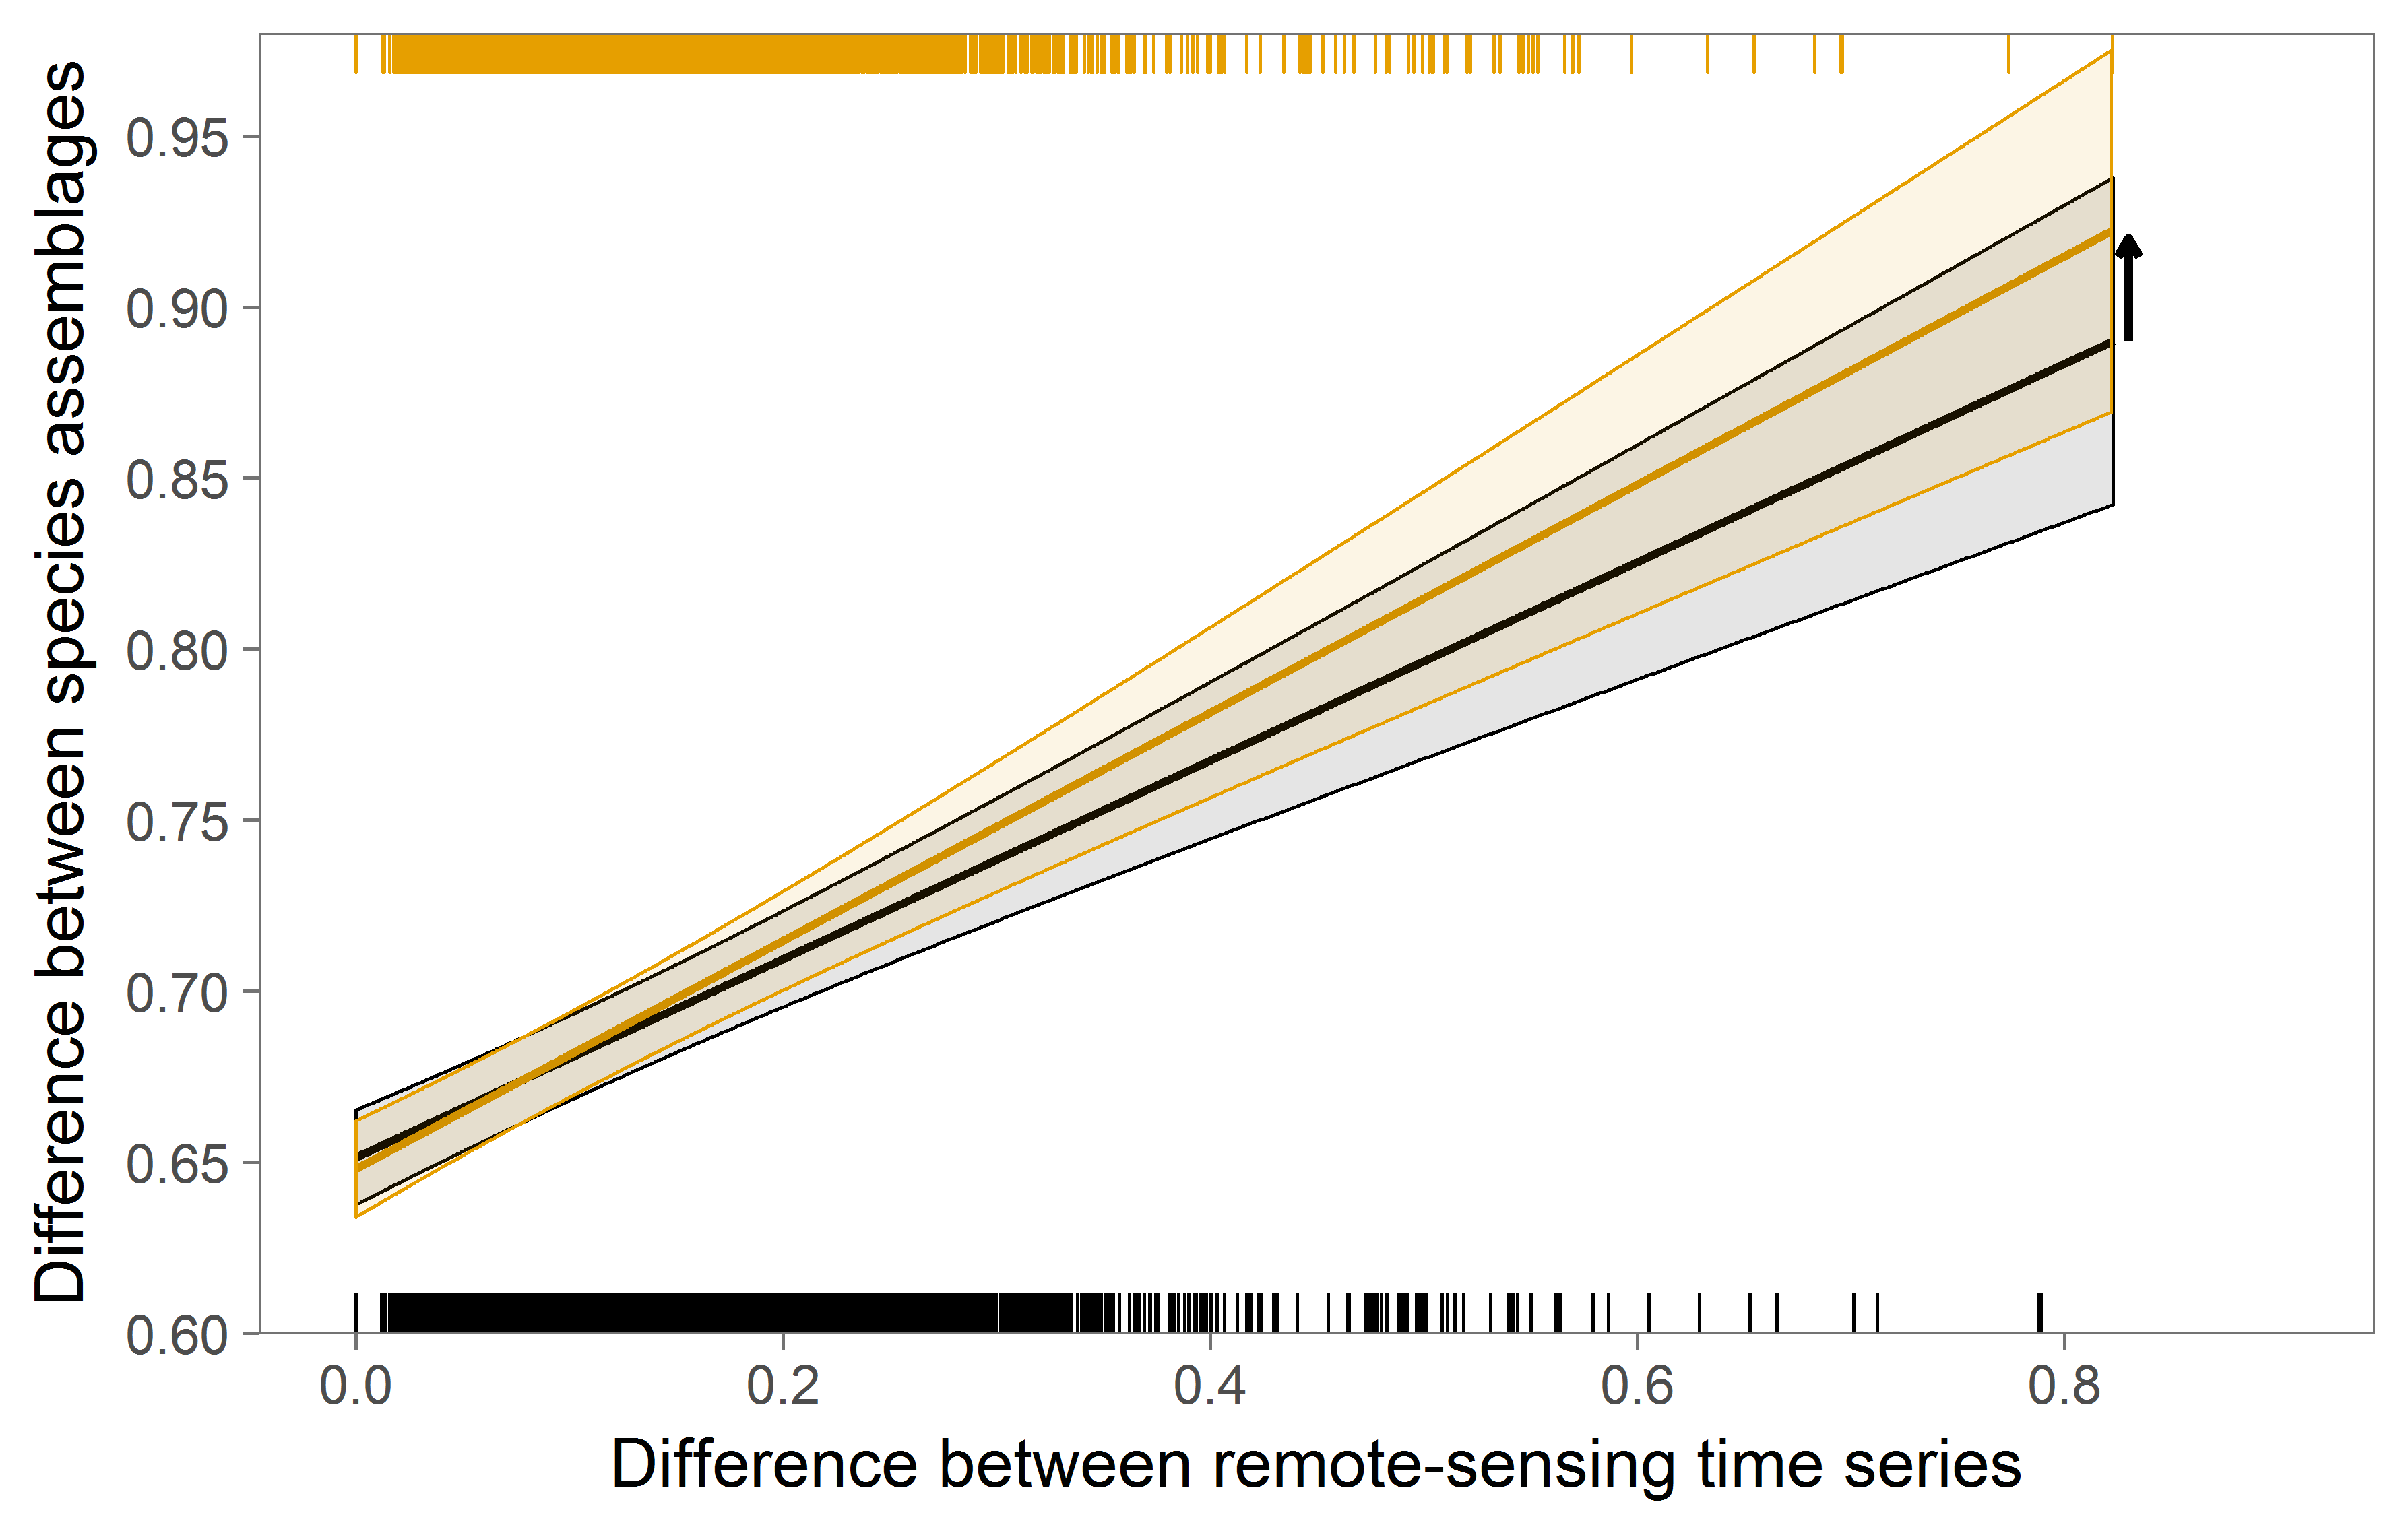
\includegraphics[width=1\textwidth]{chapter2/F02}
\caption{Shows the estimated influence of current (black) and past (orange; assessed over the past five years) BC\textunderscript{EVI} on differences in species assemblages (N = 198 studies). Rugs show the distribution of values from a single randomly selected permutation. The difference between the slopes (arrow) is the relative influence (as ratio) shown in Figures 3-6. Shading shows the predicted standard error.}
\label{F02_02}
\end{figure}
% -------------------------------------------- %

Estimating pairwise comparisons in any regression model would imply substantial pseudo-replication. To account for this, we took the subdiagonal of 100 permuted site-by-site matrices (Appendix Figure \ref{SI02_03}) to construct the GLMMs of 100 separate permutations. This ensures that for each fitted GLMM, our pairwise comparisons are mutually independent subsets \citep{Longacre2005,Newbold2016}. Fixed effects and standard errors for both current and past BC\textunderscript{EVI} were averaged across all permutations. Furthermore, for each model we calculated a marginal and conditional pseudo R-square \citep{Nakagawa2013} and significance estimate \cite{Halekoh2014}, and averaged them across all permutations. As for the fixed effects and precision estimates, the differences in explained marginal variance of past BC\textunderscript{EVI} were assessed relative to the explained marginal variance of current BC\textunderscript{EVI}.

All analyses were performed in R \citep[ver 3.2.2]{RTeam2014} using lme4 \citep[ver. 1.10]{Bolker2009,lme4} for modelling, and vegan \citep[ver. 2.2.3]{Oksanen2015} for the BC calculation of species assemblages data. The processed MODIS data and R-code for the analyses are available on GitHub (\href{https://github.com/Martin-Jung/PastLandSurfaceConditions}{https://github.com/Martin-Jung/PastLandSurfaceConditions}). 

\section{Results}
\label{C02_03}
The compositional dissimilarity of species assemblages (BC\textunderscript{Biodiversity}) increased with between-site dissimilarity in current and past photosynthetic activity (BC\textunderscript{EVI}; current: $\beta$ = 0.289, $\beta_{SE}$ = 0.063, p < 0.001; past yr\textunderscript{1:5}: $\beta$ = 0.334, $\beta_{SE}$ = 0.07, p < 0.001; Figure \ref{F02_02}, Appendix Figure \ref{SI02_05}). When the influence of past BC\textunderscript{EVI} was assessed relative to current BC\textunderscript{EVI}, the BC\textunderscript{Biodiversity} between sites was more pronounced – although the imprecision also increased - when longer time periods (of up to five years) of past BC\textunderscript{EVI} were considered (Figure \ref{F02_03}). Furthermore, the consideration of past BC\textunderscript{EVI} calculated up to five years prior to current BC\textunderscript{EVI} increased the relative explained marginal variance by 16.7\% (Appendix Table \ref{SIT02_01}). We ensured that the BC index was robust with regards to varying time period lengths (Appendix Figure \ref{SI02_06}), spatial autocorrelation (Appendix Figure \ref{SI02_07}) and other temporal and geographic biases (Appendix Figure \ref{SI02_08}). Similar results were found by using a different metric of species assemblage composition, the S\o rensen similarity index, that does not require species abundance estimates (Appendix Figure \ref{SI02_09}).

% ---------------- Figure 3 --------------------- %
\begin{figure}[ht]
\centering
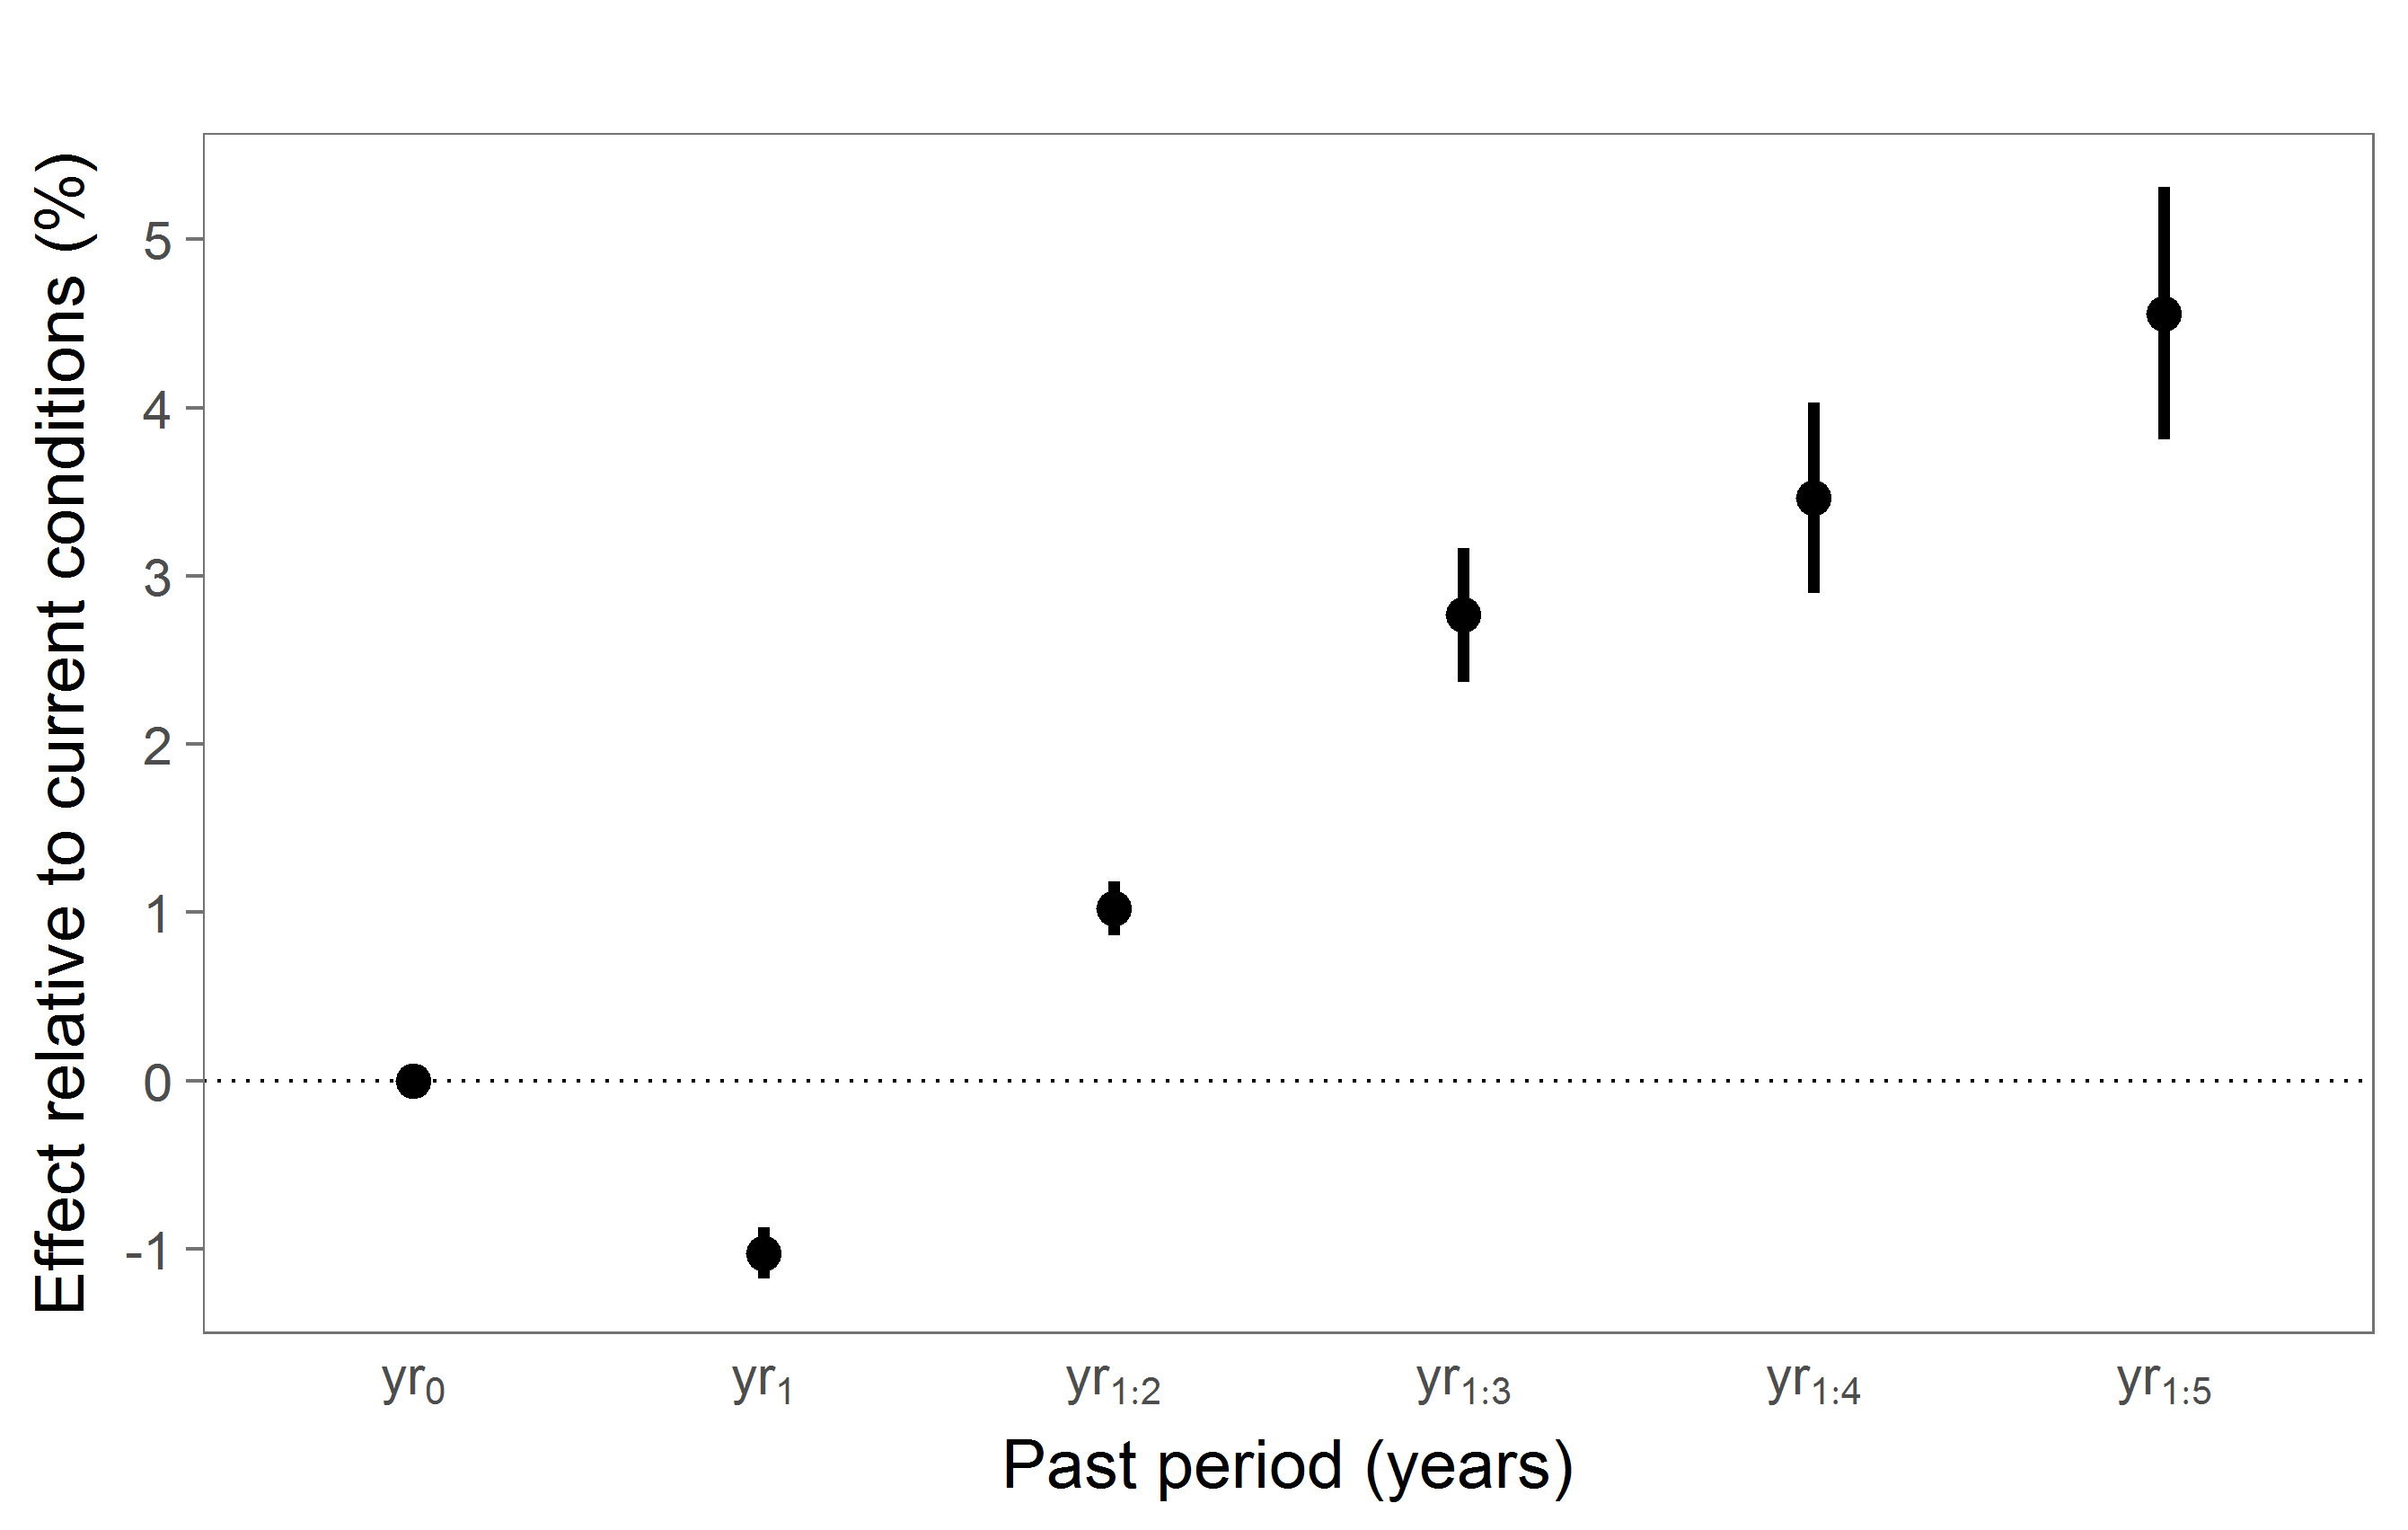
\includegraphics[width=1\textwidth]{chapter2/F03}
\caption{Overall influence on species assemblage composition of past BC\textunderscript{EVI} relative to current BC\textunderscript{EVI}, estimated individually for past periods of differing length (yr\textunderscript{1} to yr\textunderscript{1:5}, representing 1 year and up to 5 years current BC\textunderscript{EVI}). The predicted effects and their precision (standard error) of past BC\textunderscript{EVI} (yr\textunderscript{1:5}) on dissimilarity in species assemblages were transformed relative to the effects and precision of current BC\textunderscript{EVI} (yr\textunderscript{0}). Note that error bars indicate the predicted precision of differences in past BC\textunderscript{EVI} relative to the precision of differences in current BC\textunderscript{EVI}. Positive values indicate that differences in past BC\textunderscript{EVI} lead to greater differences in species assemblages than differences in current BC\textunderscript{EVI}.}
\label{F02_03}
\end{figure}
% -------------------------------------------- %
The influence of past BC\textunderscript{EVI} on species assemblages was found to vary among taxonomic groups and time periods considered (Figure \ref{F02_04}). Dissimilarity in plant, invertebrate, reptilian and bird assemblage composition increased with increasing BC\textunderscript{EVI} of the past two to five years. In contrast, the influence of past BC\textunderscript{EVI} on mammalian assemblages was greatest for the first two years relative to the influence of current BC\textunderscript{EVI} but decreased when longer periods of three to five years of past BC\textunderscript{EVI} were considered. Meanwhile, amphibian assemblages were more influenced by current than past BC\textunderscript{EVI} between sites (Figure \ref{F02_04}).
% ---------------- Figure 4 --------------------- %
\begin{figure}[ht]
\centering
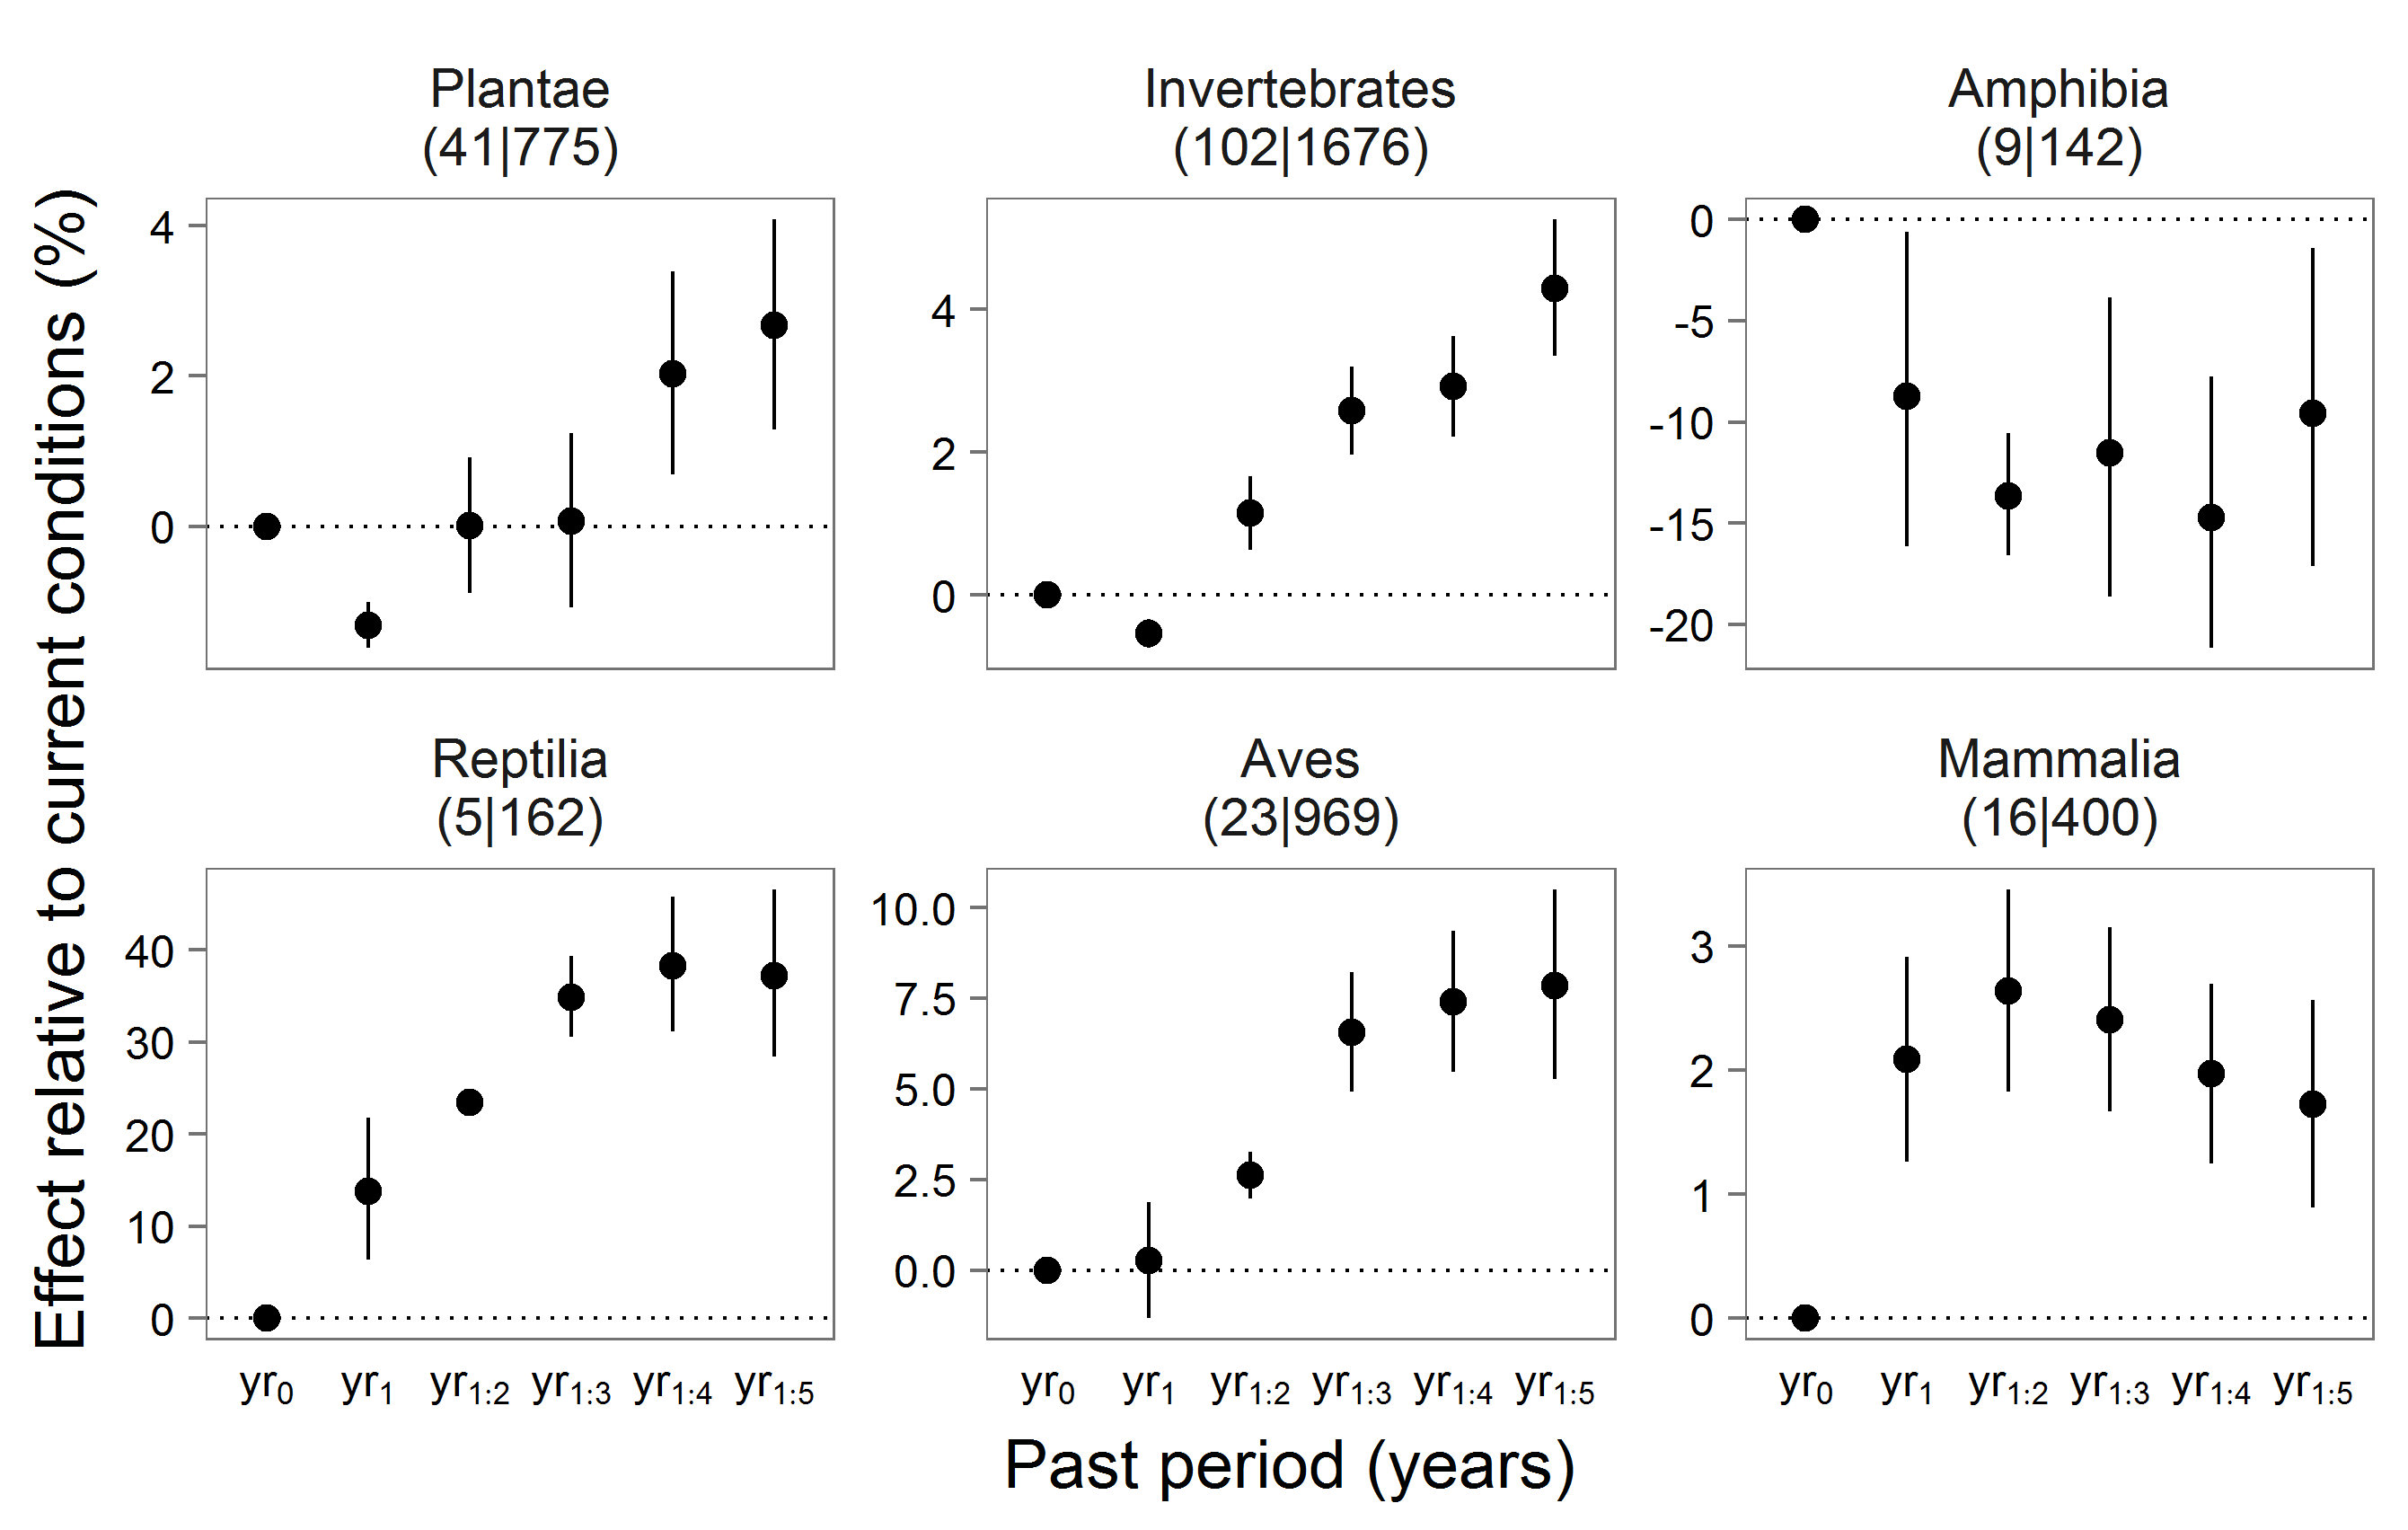
\includegraphics[width=1\textwidth]{chapter2/F04}
\caption{Influence of past BC\textunderscript{EVI} on species assemblage composition across different taxonomic groups. Visualized as relative influence of past BC\textunderscript{EVI} compared to current BC\textunderscript{EVI} as described in Figure \ref{F02_03}. The number of studies and contributing sites (N | N\textunderscript{Sites}) is indicated for each group.}
\label{F02_04}
\end{figure}
% -------------------------------------------- %
The influence of past BC\textunderscript{EVI} differed with respect to body size (Figure \ref{F02_05}). Species assemblages that were dominated by small- (> 0-9 g body mass) and medium-sized (10-99 g) mammals were more influenced by differences in BC\textunderscript{EVI} over the past one to three years, while the influence on assemblages dominated by larger ($\geq$ 100 g) mammals increased with longer time periods. Compared to assemblages dominated by medium-sized birds, assemblages of large bird species were up to five times more influenced by past relative to current BC\textunderscript{EVI}. For plant assemblages with available information on size, we found that assemblages dominated by medium-sized plants were more influenced by past BC\textunderscript{EVI} compared to those assemblages dominated by larger plant species (Figure \ref{F02_05}). 
% ---------------- Figure 5 --------------------- %
\begin{figure}[ht]
\centering
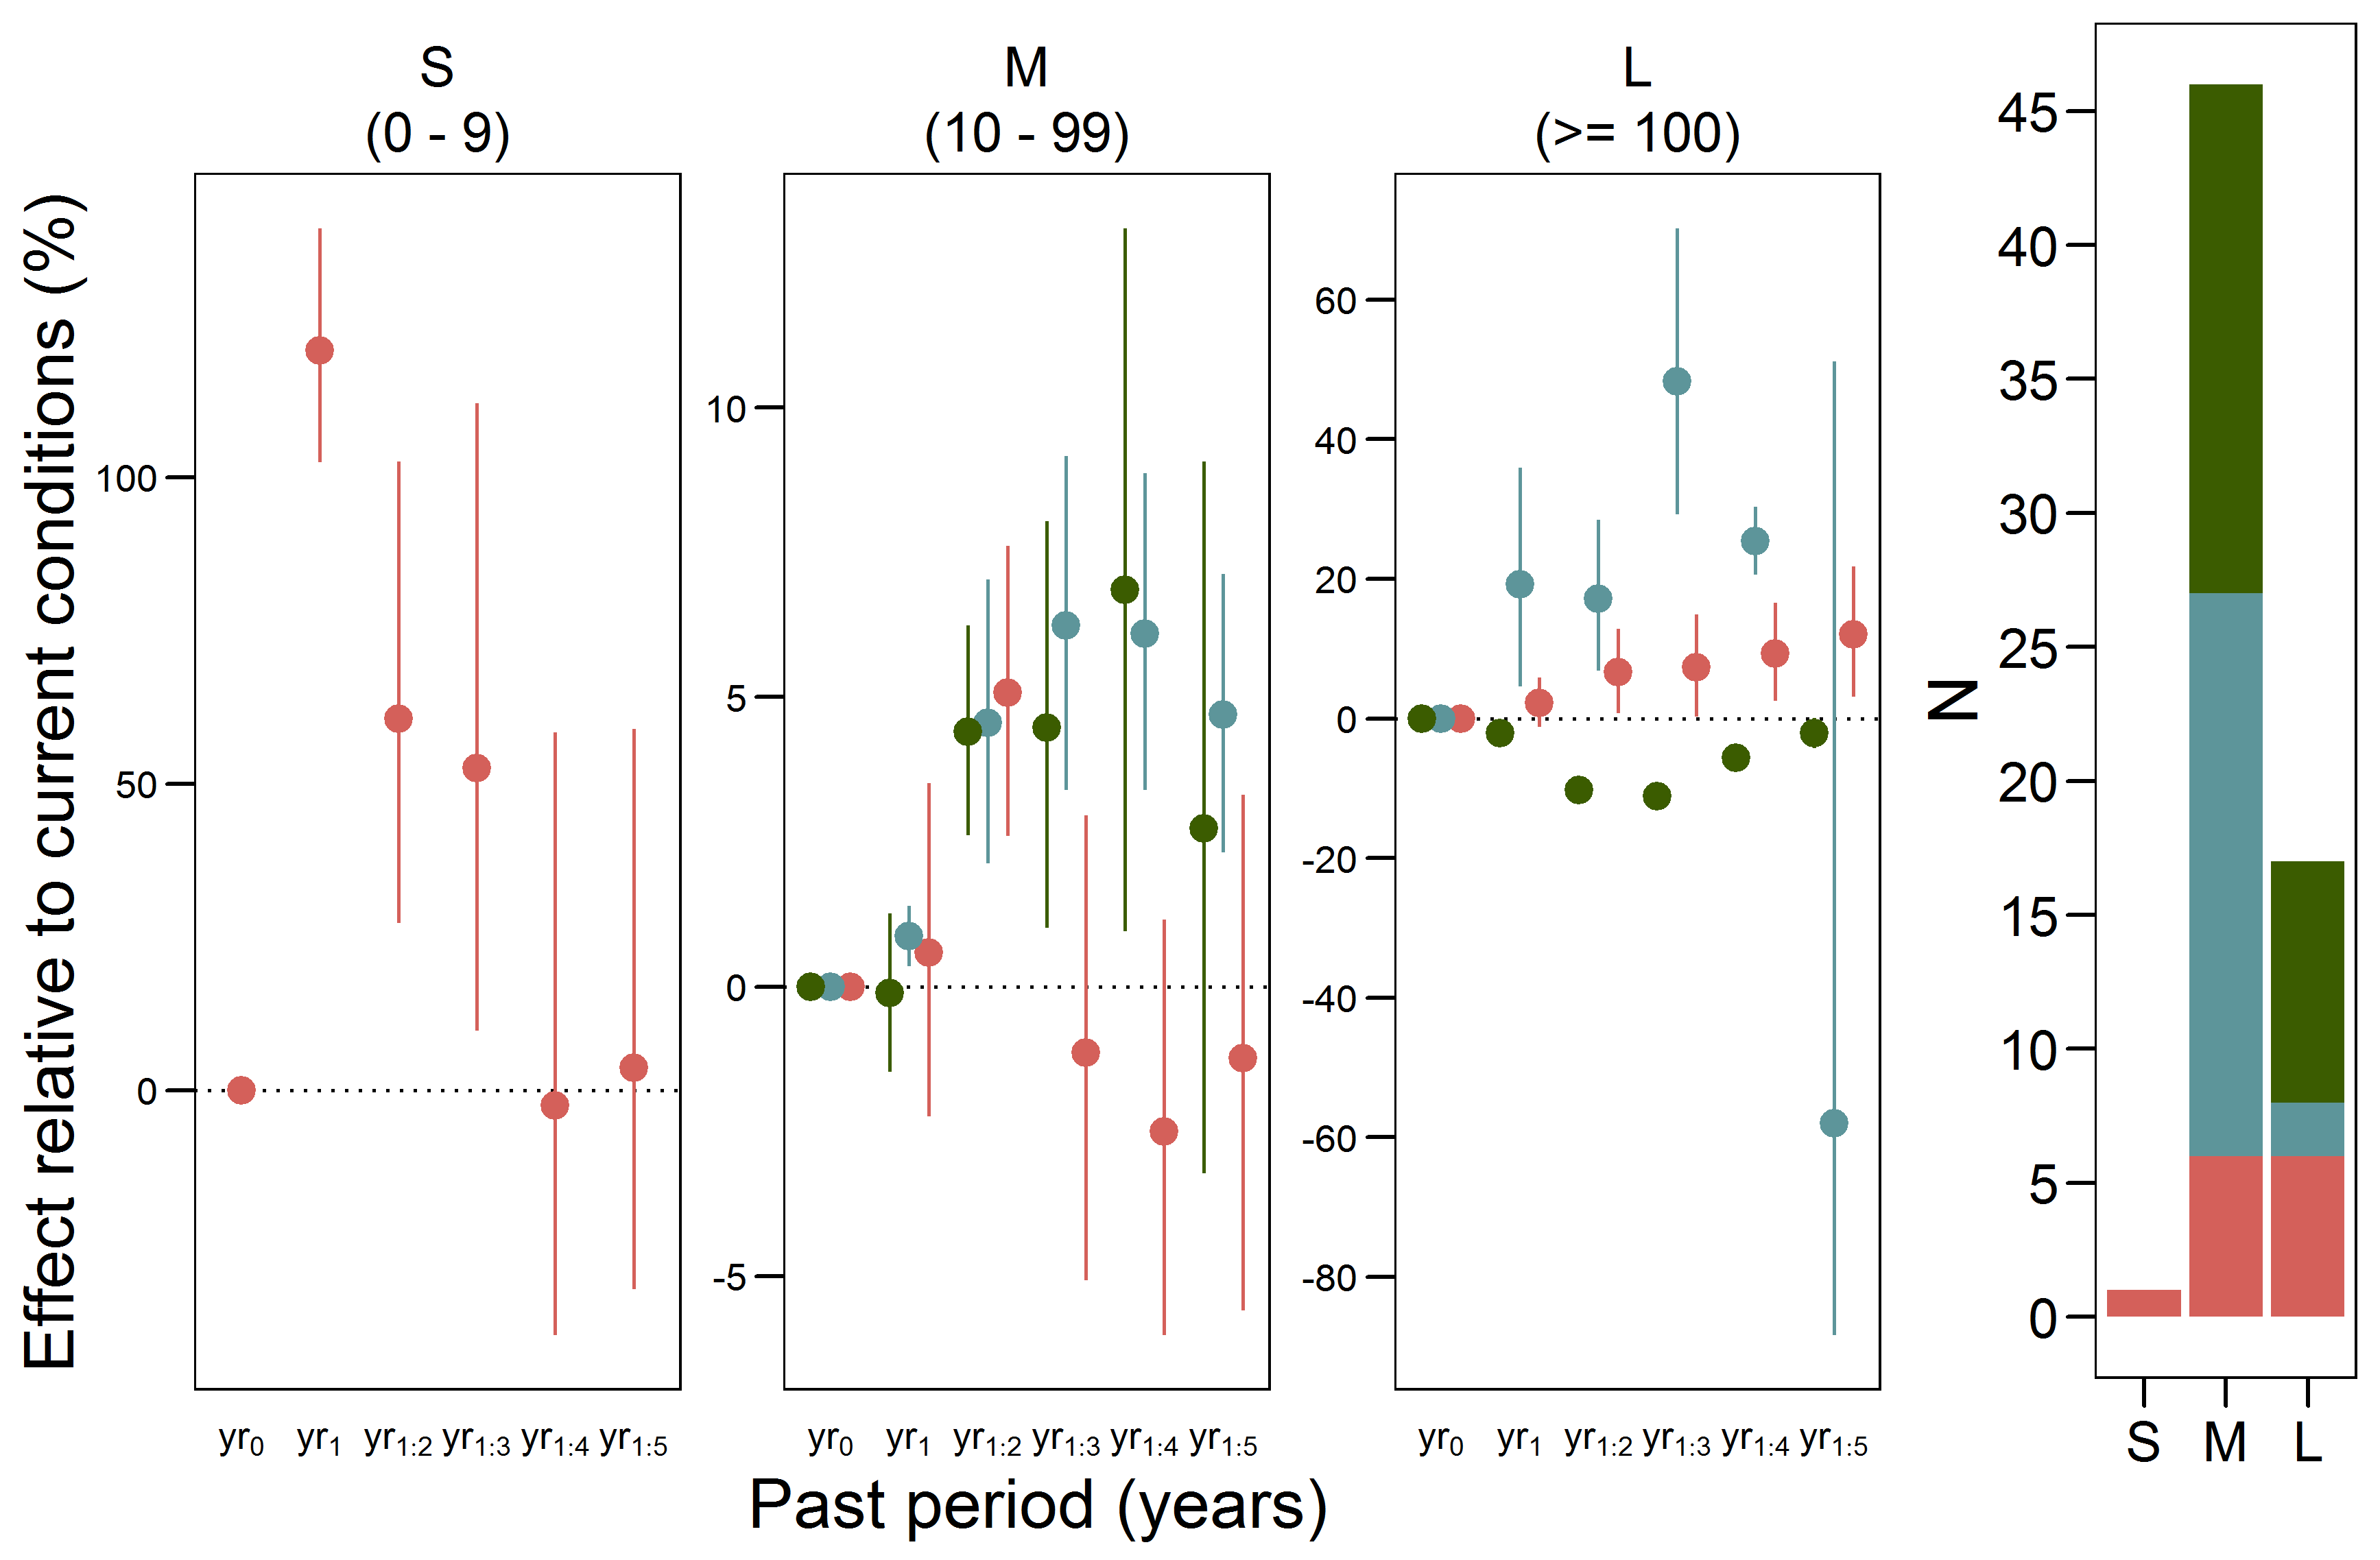
\includegraphics[width=1\textwidth]{chapter2/F05}
\caption{Influence of past BC\textunderscript{EVI} on species assemblages (N = 65) of predominantly small (> 0 - 9), medium (10 - 99) and large sized animals and plants ($\geq$ 100). Available size was measured as adult body mass (in g) for all birds (blue) and mammals (red) and height for plants (green, in cm). Within each study all species were binned into one size group and the study categorized based on which size group is predominant across all sites. The bar chart shows the number of studies that contributed to each taxonomic group and body size bin. Visualized as relative influence of past BC\textunderscript{EVI} compared to current BC\textunderscript{EVI} as described in Figure \ref{F02_03} and methods.}
\label{F02_05}
\end{figure}
% -------------------------------------------- %
Differences among trophic levels were also seen in the influence of past BC\textunderscript{EVI} on BC\textunderscript{Biodiversity} and increased with longer time periods considered (Figure \ref{F02_06}). Species assemblages dominated by omnivorous and herbivorous assemblages were more influenced by past BC\textunderscript{EVI} of even one year relative to the influence of current BC\textunderscript{EVI}, while detritivores assemblages were only more influenced by past BC\textunderscript{EVI} if periods of the past three years were considered (Figure \ref{F02_06}). In contrast, studies with predominantly carnivorous species were more influenced by current BC\textunderscript{EVI} and showed no overall trend with longer time periods of past BC\textunderscript{EVI} considered (Figure \ref{F02_06}). 
% ---------------- Figure 6 --------------------- %
\begin{figure}[ht]
\centering
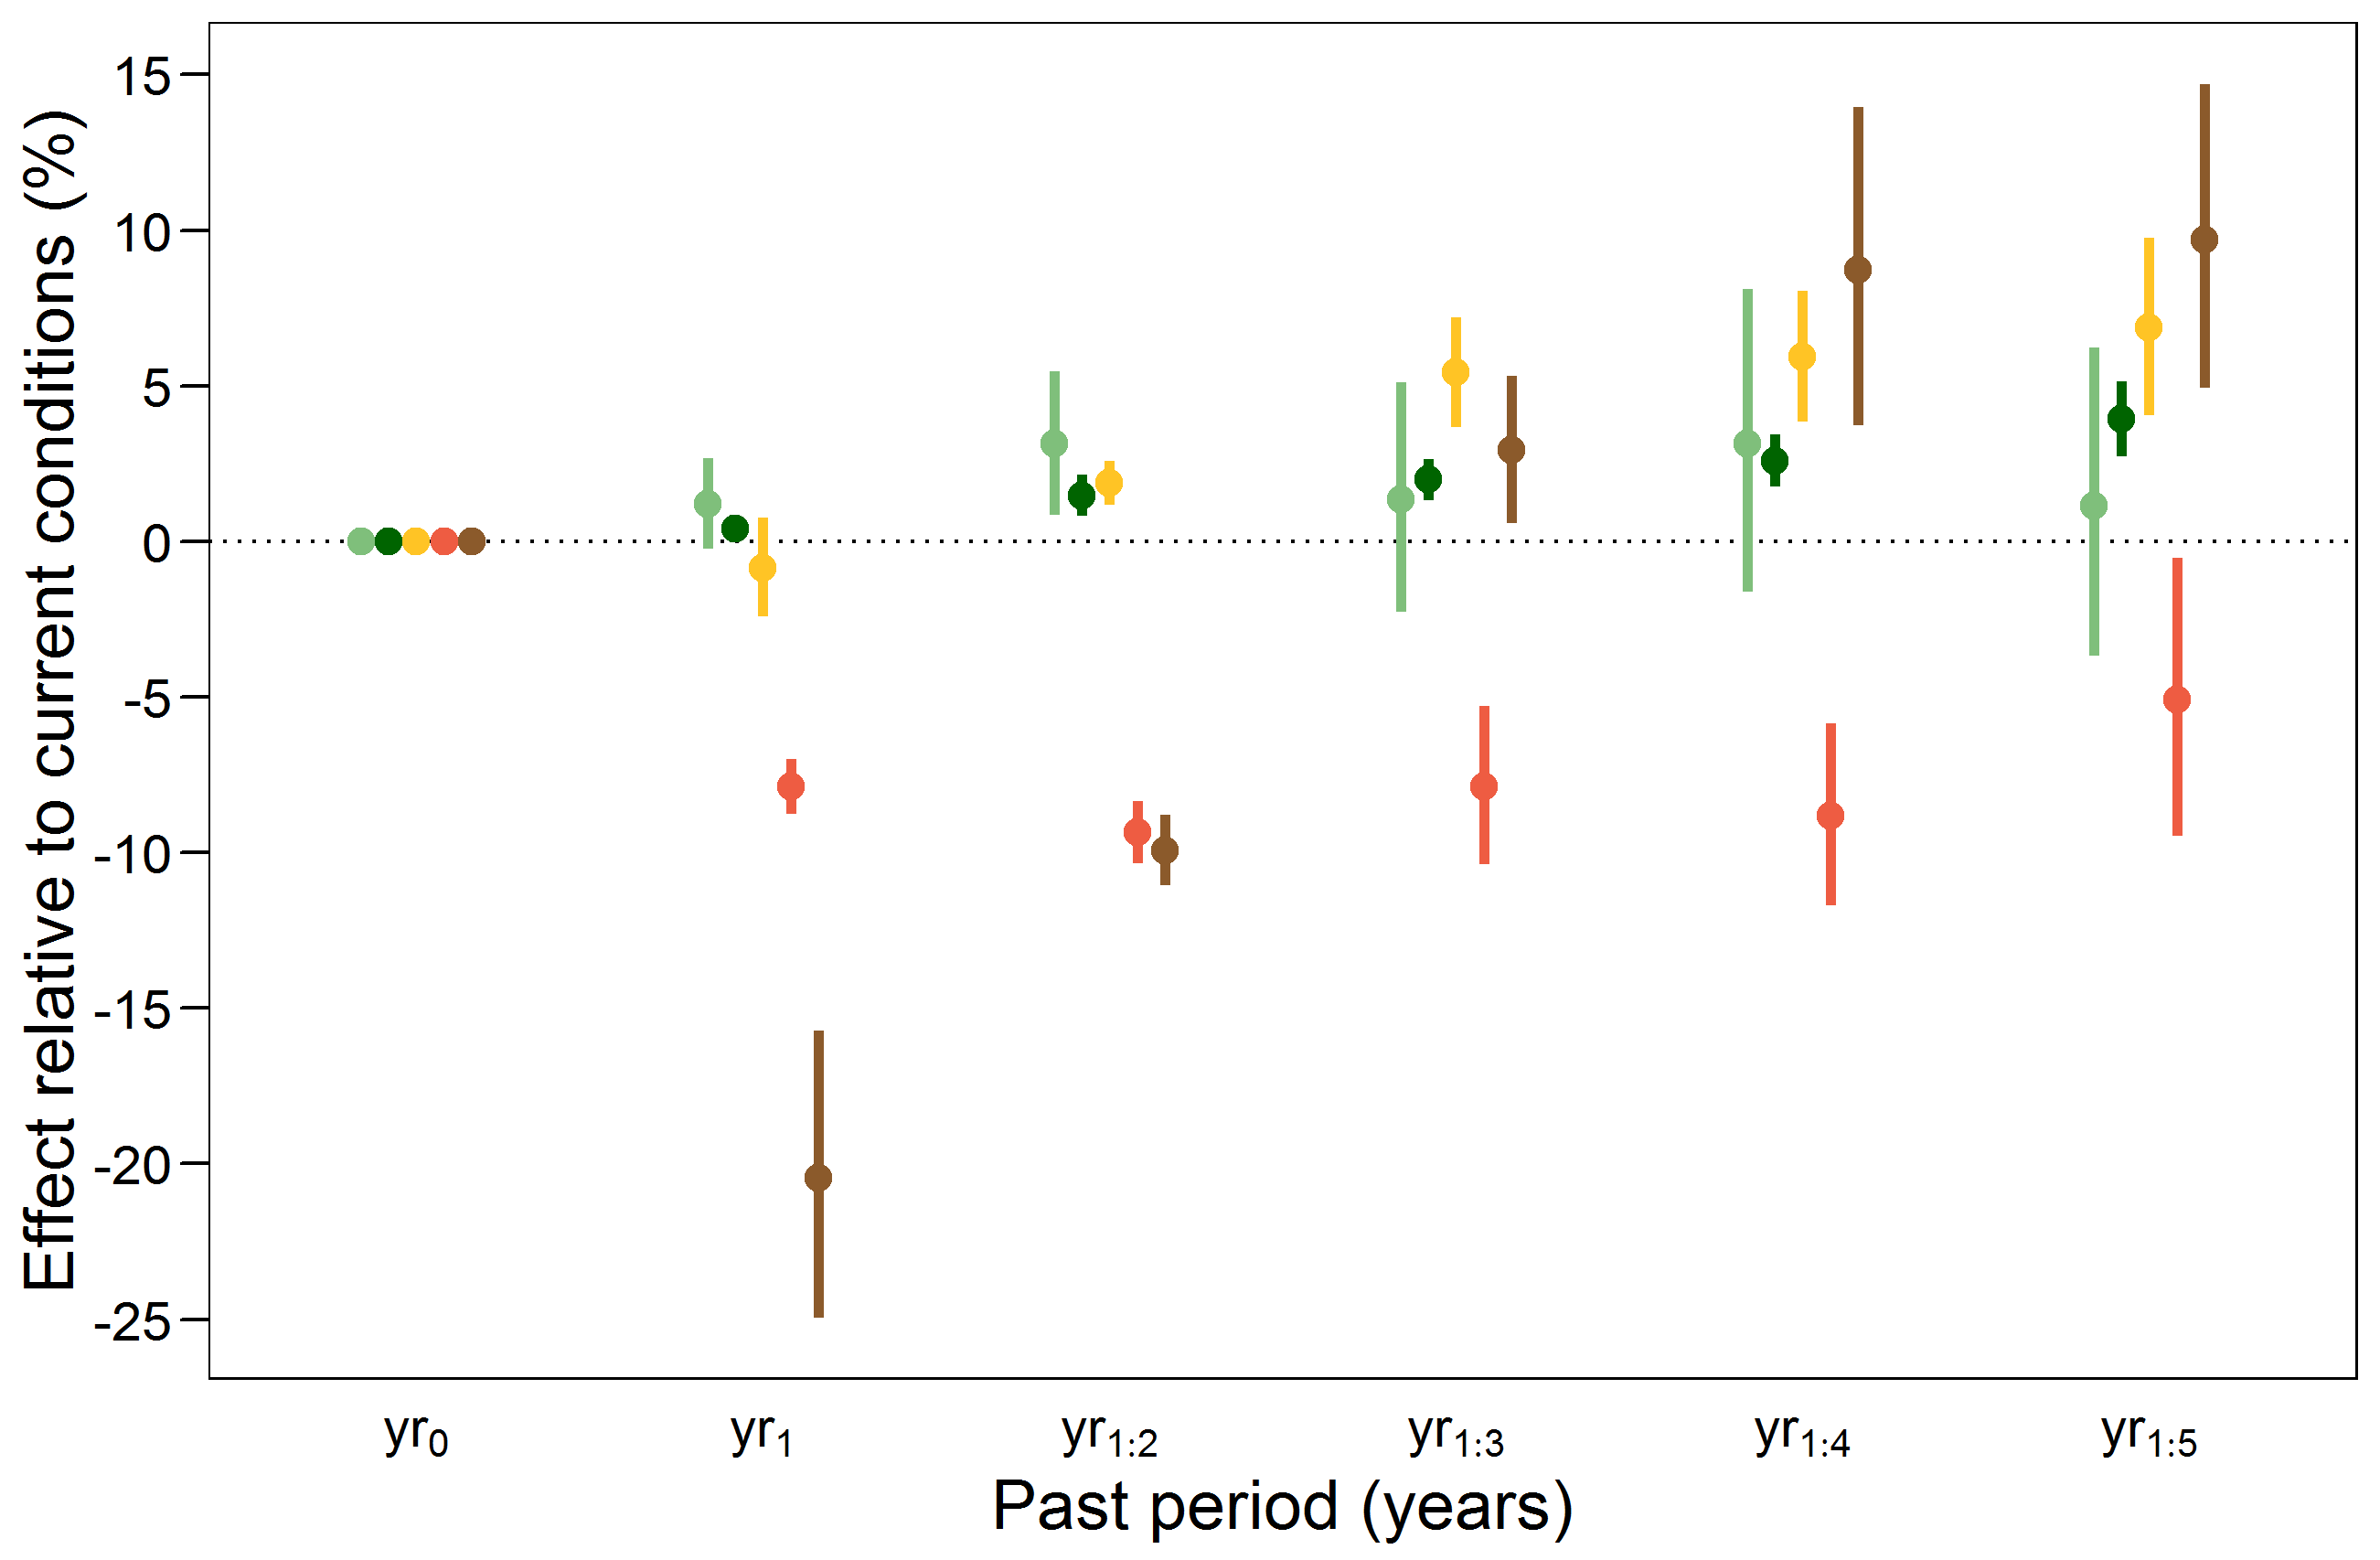
\includegraphics[width=1\textwidth]{chapter2/F06}
\caption{Influence of past BC\textunderscript{EVI} on trophic bins across studies (N = 130). Within each study all species were categorized as one trophic level and the study categorized based on which level is predominant across all sites. Colours indicate the influence of current and past BC\textunderscript{EVI} for autotroph plants (light green, N=28), herbivores (dark green, N=49), omnivores (yellow, N= 29), carnivores (red, N=13) and detritivores (brown, N=9). Visualized as relative influence of past BC\textunderscript{EVI} compared to current BC\textunderscript{EVI} as described in Figure \ref{F02_03}.}
\label{F02_06}
\end{figure}
% -------------------------------------------- %

\section{Discussion}
\label{C02_04}
The main aim of this study was to investigate if between-site dissimilarity in current and past photosynthetic activity of vegetation (BC\textunderscript{EVI}) can predict compositional dissimilarity in sites’ species assemblages (BC\textunderscript{Biodiversity}). In contrast to previous PREDICTS-based studies that used discrete measures of current land use and land-use intensity \citep{Newbold2015,Newbold2016}, we used a continuous measure of between-site dissimilarity in remotely-sensed photosynthetic activity that summarises (inter- and intra-annual) vegetation dynamics in a single metric (the BC\textunderscript{EVI}). We explicitly differentiated between current (the full year prior to species assemblage sampling) and past BC\textunderscript{EVI} (periods of up to five years before current) that could have influenced compositional dissimilarity in species assemblages. Similar to previous studies using the same dataset to analyse compositional differences with respect to land use \citep{Newbold2016}, we found that sites with more different current BC\textunderscript{EVI} also had more different species assemblages (Figure \ref{F02_02}, Appendix Figure \ref{F02_05}). However, the BC\textunderscript{EVI} calculated over five years prior to biodiversity sampling had, on average, an even greater influence on between-site dissimilarity in species assemblage composition compared to current BC\textunderscript{EVI} (Figure \ref{F02_03}). This pattern was consistent across most taxonomic (Figure \ref{F02_04}) and functional groups (Figure \ref{F02_05} and \ref{F02_06}). Here we discuss potential causes and implications of the observed patterns as well as factors that can affect the BC\textunderscript{EVI}.

\subsection{Potential drivers of dissimilarities in photosynthetic activity}
\label{C02_0401}
Dissimilarities in photosynthetic activity can be caused by many natural \citep{Fensholt2012,Zhu2016} and/or anthropogenic factors \citep{Lambin2006,Turner2007}. The latter were likely the dominant cause of current differences between sites in our analyses, given that the PREDICTS database includes only studies of mostly small geographic extent with a difference in current human land use or land-use intensity \citep{Hudson2016}, however climatic factors likely influence the BC\textunderscript{EVI} as well. Dissimilarity metrics of photosynthetic activity can be considered a coarse approximation of overall differences in land use and land cover as well as in climatic and other abiotic factors between sites \citep{Linderman2005,Lupo2007,Lhermitte2011}. Past studies have linked differences in vegetation dynamics with the use intensity of agriculture \citep{Estel2015,Tong2017}, land-cover change such as deforestation events  \citep{Lambin1994,DeVries2015b}, or land degradation and intensification \citep{DeJong2011,Muller2014}. The BC\textunderscript{EVI}, similar to other metrics used to monitor remotely-sensed vegetation dynamics \citep{Linderman2005,Rowhani2008,Lhermitte2011}, quantifies dissimilarity in photosynthetic activity across different types of land cover, by exploiting both distance between time series (the absolute difference in EVI data) and amount (area under the time series) of photosynthetic activity. Besides differences in land use and land cover, dissimilarity metrics such as the BC\textunderscript{EVI} will also be affected by climatic differences in precipitation and radiation \citep{Fensholt2012,Zhu2016}, soil properties \citep{Ahmed2017} or plant species composition \citep{He2009}. The BC\textunderscript{EVI} thus quantifies dissimilarity in vegetation dynamics caused by both natural and anthropogenic factors affecting EVI time-series.

However, some natural and anthropogenic factors cannot be directly quantified from remotely-sensed time series \citep{Peres2006,Turner2007} and the BC\textunderscript{EVI} is limited to those aspects that affect photosynthetic activity of vegetation. Furthermore, because of the way the BC\textunderscript{EVI} is calculated, it can only represent overall dissimilarity in photosynthetic activity but cannot be used to infer directionality or timing of change (vegetation regrowth or loss, disturbances such as fires, etc.). By using entire periods (\ie five full years, instead of the fifth year) it is not possible to disentangle overall dissimilarity and any ‘change’ in photosynthetic activity \textit{per se} \citep[cf.][]{Linderman2005}. Calculating the BC\textunderscript{EVI} index on longer time periods did not affect the possible range of observed values (Appendix Figure \ref{SI02_06}), however it likely enhances our ability to capture aspects of past variability in vegetation dynamics caused by either natural and/or anthropogenic drivers. We recommend that future studies evaluate the performance of the BC\textunderscript{EVI} relative to other time-series dissimilarity metrics. 

\subsection{Influences of current and past dissimilarities in photosynthetic activity on biodiversity}
\label{C02_0402}
Our results suggest that species assemblage composition was consistently more dissimilar between sites with greater current dissimilarity in photosynthetic activity of vegetation (as quantified by the BC\textunderscript{EVI}) (Figure \ref{F02_02}, Appendix Figure \ref{F02_05}). This is in line with previous studies that have correlated some measurement of dissimilarity in current ‘environmental heterogeneity’ with compositional dissimilarity in species assemblage composition \citep{Buckley2008,He2009,Newbold2016}. However species assemblages might also be explicitly influenced by past dissimilarity in photosynthetic activity \citep{Johnson2008,Watson2014,Ogle2015,Perring2015}. 

Differences in past BC\textunderscript{EVI} were on average more correlated with dissimilarity in species assemblages than differences in current BC\textunderscript{EVI} (Figure \ref{F02_02}-\ref{F02_03}). This could indicate that past dissimilarity in photosynthetic activity continues to have a lasting influence or memory effect on species assemblages \citep{Ogle2015}, especially as the effect generally increased as longer periods of past BC\textunderscript{EVI} were considered (Figure \ref{F02_03}), therefore increasing the likelihood that past changes in photosynthetic activity of vegetation have been captured. Longer periods of past BC\textunderscript{EVI} also increased the explained marginal variance (Appendix Table \ref{SIT02_01}), although most of the variance was already explained by differences in study identity (thus by sampling methods and local factors). The marginal variance explained was modest, but comparable to other broad-scale studies using the same species assemblage dataset \citep{Newbold2014b,DePalma2015,Jung2016}. It is a limitation that we used data from a wide variety of sources \citep{Hudson2016}, which were typically not designed to study lag or memory effects of past changes in land-surface conditions such as photosynthetic activity. At many of the sites in our analyses inter-annual photosynthetic activity could have remained relatively stable during the past five years, which would reduce our ability to differentiate any effects of past BC\textunderscript{EVI}. Similarly, any dissimilarity in photosynthetic activity among pairs of sites could have been even greater before the monitoring period of MODIS (since year 2000), which we were unable to quantify using these data. 

Notably, species assemblages of some taxonomic groups were more dissimilar in composition than others if past dissimilarity in photosynthetic activity was considered (Figure \ref{F02_04}). The influence of past BC\textunderscript{EVI} on reptilian species assemblages was large (\textasciitilde35\% more different than current) even for the relatively short period of five years (Figure \ref{F02_04}). Potentially many of the sites of the reptilian studies have been subjected to relatively recent changes in photosynthetic activity of vegetation prior to species assemblage sampling. Indeed, in one of the studies, \cite{Woinarski2009} explicitly suggested an influence of past fires and varying grazing intensity on reptilian species assemblages. In contrast, we found that amphibian species assemblages were less influenced by past compared to current BC\textunderscript{EVI}, despite being more influenced by current BC\textunderscript{EVI} than all other taxonomic groups (Appendix Figure \ref{F02_05}). An explanation could be that most compositional differences between amphibian assemblages that are attributable to past dissimilarities in photosynthetic activity are already explained by current dissimilarity in BC\textunderscript{EVI}. It may be that amphibian assemblages are more influenced by factors other than past photosynthetic activity (such as microclimatic conditions). Disentangling broad taxonomic groups into functional groups may assist in highlighting specific responses to past dissimilarities in photosynthetic activity.

Differences in functional traits can influence species responses to dissimilarity in photosynthetic activity \citep{Newbold2013,DePalma2015} and we expect that on average smaller species would be more affected by recent dissimilarity in photosynthetic activity (a few years before sampling). Our results confirm this assumption as species assemblages with predominantly small- or medium-sized plants, birds and mammals were relatively more influenced by past BC\textunderscript{EVI} over two to three years prior to sampling than by current BC\textunderscript{EVI} (Figure \ref{F02_05}). Smaller species tend to live shorter lives and disperse less far than larger species \citep{Brown2004,Thomson2011,Stevens2014}, which might make them more susceptible to dissimilarity in photosynthetic activity shortly before sampling \citep{Watson2014}. Similar to previous studies \citep{Jakovac2016} we showed that smaller plant species were more influenced by past dissimilarity in photosynthetic activity over up to five years prior to sampling as quantified by the BC\textunderscript{EVI} (Figure \ref{F02_05}). For assemblages dominated by larger plants we did not detect such an influence and it is likely that the considered period (five years) was too short to show measurable influences. Overall our results indicate that assemblages dominated by smaller species might have been more influenced by past dissimilarity in photosynthetic activity,  possibly because of carry-over or ecological memory effects \citep{Harrison2011,Ogle2015}. Other functional traits, such as generation time or dispersal capability \citep{Watson2014}, as well as better coverage of existing traits for underrepresented taxonomic groups could assist in further disentangling these influences especially given the large uncertainty across most influences (Figure \ref{F02_05}). 

The response of species assemblages to dissimilarities in past photosynthetic activity also differed between trophic bins. Except for carnivores, species assemblage composition of all trophic bins were on average more influenced by longer periods of past rather than by current dissimilarity in photosynthetic activity, as measured by BC\textunderscript{EVI} (Figure \ref{F02_06}). Yet we found noticeable lags in the observed influence of past BC\textunderscript{EVI} with varying time periods. Relative to the influence of current BC\textunderscript{EVI}, the influence of past BC\textunderscript{EVI} was larger for assemblages dominated by autotrophs, herbivores, omnivores and detritivores (Figure \ref{F02_06}). Notably, detritivores were more correlated with past BC\textunderscript{EVI} only if past periods of three to four years were considered. This supports previous studies which have shown that plant-dependant species are highly sensitive to variability in current and past photosynthetic activity as quantified by remote sensing \citep{Pettorelli2006,Newton2014}. In contrast, we found predominantly carnivorous assemblages to be less influenced by past BC\textunderscript{EVI} compared to current BC\textunderscript{EVI} regardless of the considered time period. Possibly, carnivore abundance was more influenced by contemporary prey density \citep{Terborgh2015} than past dissimilarity in photosynthetic activity (Figure \ref{F02_06}). Because of a lack of data for carnivores and herbivores co-occurring at the same site, we were unable to investigate such interactions. 

\section{Study implications and conclusions}
\label{C02_05}
Knowledge about past dissimilarities in land-surface conditions, such as photosynthetic activity, and their influence on species assemblages is important for both the design of ecological studies and interpretation of dissimilarities in current composition of species assemblages. We found that sites with more dissimilar past than current photosynthetic activity (as quantified by the BC\textunderscript{EVI}) were more strongly correlated with compositional dissimilarity in local species assemblages among spatial pairs of nearby sites. Ignoring such past influences can lead to biased biodiversity estimates by not accounting for extinction debts or immigration credits still to be paid \citep[see ][]{Tilman1994} or lasting ecological memory and carry-over effects because of higher variability in past photosynthetic activity \citep{Rowhani2008,Cole2015,Ogle2015}. We suggest that future broad scale studies investigating biodiversity responses to environmental changes should explicitly consider legacy effects that influence species assemblages in a study area and we demonstrate how remote sensing can help to quantify such effects globally. Our approach could be extended to incorporate differences in the vegetation dynamics of the surrounding landscape. There is some evidence that landscape-wide temporal differences in photosynthetic activity can affect species assemblage composition in the wider landscape \citep{Manning2009,Fernandez2016}. In conclusion, we have demonstrated that compositional dissimilarity of species assemblages, of various taxonomic and functional groups, are not only influenced by dissimilarity in current photosynthetic activity, but also by dissimilarity in past photosynthetic activity over the last five years. Future studies should investigate the influence of disturbance events and directionality of changes in photosynthetic activity for more than five years before local biodiversity sampling.

%\section{Acknowledgements}
%\label{C02_06}
%We thank all PREDICTS data contributors for their biodiversity data, which was collated using support from the Natural Environment Research Council (NERC, grant number: NE/J011193/2). PREDICTS is endorsed by the GEO BON. This study has benefited from publicly available data from the TRY initiative on plant traits (\href{http://www.try-db.org}{http://www.try-db.org}). We acknowledge the University of Sussex, School of Life Sciences for a doctoral training grant and for providing computing facilities.

\section{Data availability}
\label{C02_06}
Extracted MODIS data and pairwise biodiversity permutations are available on GitHub. A 2016 snapshot of the PREDICTS database has been openly released earlier (\href{http://dx.doi.org/10.5519/0066354}{http://dx.doi.org/10.5519/0066354}).

\clearpage
%\bibliography{content/01Chapter}

%\appendix
%\begingroup
%  Blank

%\endgroup

\endgroup

%---------------------------------------------------
% APPENDICES
%---------------------------------------------------
%\appendix
%\begingroup
%  \input{content/Chapter01}
%\endgroup
%\backmatter
%\input{front/Acronyms.tex}

%---------------------------------------------------
% BIBLIOGRAPHY
%---------------------------------------------------
%\clearpage
%\phantomsection
%\bibliography{Chapters/bibliography}
%\clearpage\pagestyle{empty}
\pdfbookmark[0]{Colophon}{colophon}
\hfill

\vfill

\begin{flushright}
Lorem ipsum dolor sit amet, consectetur adipiscing elit. Integer nec venenatis augue. Maecenas sed egestas elit, quis ultrices lacus. Maecenas hendrerit massa nisi, congue congue quam pretium eu. Proin erat quam, iaculis ac iaculis nec, rhoncus vitae tortor. Pellentesque neque eros, aliquet tincidunt enim sed, volutpat ultrices nibh. Nullam feugiat gravida velit, ut aliquam est finibus ac. Cras pharetra nibh enim, vel lacinia enim pulvinar eget. Maecenas gravida ante vitae convallis eleifend. 
\end{flushright} 


%---------------------------------------------------
% END DOCUMENT
%---------------------------------------------------
\end{document}
